%%%%%%%%%%%%%%%%%%%%%%%%%%%%%%%%%%%%%%%%%%%%%%%%%%%%%%%%%%%%%%%%%%%%%%%%%%%%%%%%
%2345678901234567890123456789012345678901234567890123456789012345678901234567890
%        1         2         3         4         5         6         7         8

\documentclass[letterpaper, 10 pt, conference]{ieeeconf}  % Comment this line out
                                                          % if you need a4paper
%\documentclass[a4paper, 10pt, conference]{ieeeconf}      % Use this line for a4
                                                          % paper

\IEEEoverridecommandlockouts                              % This command is only
                                                          % needed if you want to
                                                          % use the \thanks command
\overrideIEEEmargins
% See the \addtolength command later in the file to balance the column lengths
% on the last page of the document



% The following packages can be found on http:\\www.ctan.org
\usepackage{graphicx} % for pdf, bitmapped graphics files
%\usepackage{epsfig} % for postscript graphics files
%\usepackage{mathptmx} % assumes new font selection scheme installed
%\usepackage{times} % assumes new font selection scheme installed
%\usepackage{amsmath} % assumes amsmath package installed
%\usepackage{amssymb}  % assumes amsmath package installed
\usepackage{float}
\usepackage{listings}
\usepackage{hyperref}
\usepackage{pdfpages}

\title{\LARGE \bf
Robot Metabolism: Semester Report Spring 2021*
}
% get at least 20 citations

\author{Philippe Martin Wyder$^{1}$ Riyaan Sunil Bakhda$^{2}$ Nihar Niraj Garg$^{3}$% <-this % stops a space
\thanks{*This work partially funded by DARPA TRADES COLUM 5216104 SPONS GG012620 01 60908 HL2891 20 250}% <-this % stops a space
\thanks{$^{1}$Philippe Wyder, Doctoral Student, Mechanical Engineering,
        Columbia University, New York, NY 10027, USA
        {\tt\small www.philippewyder.com}}%
\thanks{$^{2}$Riyaan Bakhda, Bachelor of Science Student, Computer Science,
        Columbia University, New York, NY 10027, USA}%
\thanks{$^{3}$Nihar Garg, Master of Science Student, Mechanical Engineering,
        Columbia University, New York, NY 10027, USA}%
}


\begin{document}

\maketitle
\thispagestyle{empty}
\pagestyle{empty}


%%%%%%%%%%%%%%%%%%%%%%%%%%%%%%%%%%%%%%%%%%%%%%%%%%%%%%%%%%%%%%%%%%%%%%%%%%%%%%%%
\begin{abstract}

This report introduces the Robot Metabolism, a magnet-connector based truss-robot that is able to metabolize hunted or gathered links to improve itself once a manually assembled base structure has been created. The field of modular robotic research tries to develop a "generalizable" robotic building block that can be reassembled to satisfy all of our robotic needs. We aim to develop modules that automatically assemble three-dimensional structures and solve whatever task is at hand---carry a payload, build a bridge, automatically erect shelter, help with search and rescue operations, aide space exploration, and serve as a platform for exploring the origin of life. First, this report discusses existing modular robotic solutions, and introduces the most salient aspects of a modular robotics system. Second, the proposed Robot Metabolism and its design evolution are discussed in the context of the previously addressed systems. Finally, the report lays out the next steps and future design considerations.

\end{abstract}


%%%%%%%%%%%%%%%%%%%%%%%%%%%%%%%%%%%%%%%%%%%%%%%%%%%%%%%%%%%%%%%%%%%%%%%%%%%%%%%%
\section{INTRODUCTION}

Modular robots are systems consisting of multiple parts called modules, links or cells that assemble to achieve various tasks. Toshio Fukada introduced modular robotics in his conference paper at the 1988 IEEE International Conference on Robotics and Automation (ICRA), sparking a new generation of robotics research\cite{FukudaDynamicallySystem}. In the last thirty years, the field of modular robotics has grown and produced many different modular robotic systems. These robots can be categorized by a variety of criteria, from their reconfiguration behavior, attachment mechanisms, degrees of freedom (DoF), ways of locomotion, control and communication approaches. This report will address the motivation for building modular robots, introduce the key characteristics of a modular robotic system, and highlight a selected few robots that provide context for the Robot Metabolism.

The core motivations for creating modular robots is their versatility, configurability, scalability, resiliency, their potential for automatic assembly and robot topology evolution\cite{Zykov2007, Yim2009MSRR, Gilpin2010}. Reducing the complexity of a robotic system to many identical sub-modules opens up the possibility for mass producing those modules and thereby lowering the overall cost\cite{Yim2009MSRR}. The modular robotic approach detaches the resiliency of a system from the mere strength of its materials or individual components---leveraging its modularity and redundancy. Thus, on top of having redundant components, a system constructed from many identical modules can repair itself by replacing or shedding any defective modules. Similar to biological systems, a robot built from many identical cells that by them selves have little functionality could be combined to form sophisticated machines.

At the time of writing, no current robot platform comes close to its biological counterpart. The success of modular robotics is feasible given three assumptions: (1) the modular system is scaleable, (2) the modules are mass-producible and hence cheap, (3) the modules are simple. Today's modular robots do not fulfill these three criteria. Often, the modules are already too complex in themselves. Robot Metabolism is trying to change that. 


\section{Related Work}

This section will introduce the customary modular robot classifications, as well as a selected subset of robots to help-differentiate between classes. Modular robots can be classified as self-configuring or manually configured robots\cite{Stoy2010}. Self-configuring robots are capable of attaching and detaching from other modules automatically, while manually configured robots need to be assembled by an operator. Robot Metabolism is a modular self-configuring robot (MSR) that requires a triangle or tetrahedron minimal initial configuration.

\subsection{Configuration Types}
Self-configuring robots further separate into chain, lattice, and truss systems\cite{Yim2007,Gilpin2010}.

\subsubsection{Chain systems} form either chain or tree type structures, and are limited to serial connections. Mark Yim's PolyBot is an example of a pure chain system\cite{Yim2000}. In various configurations the PolyBot can overcome obstacles, move in a snake gate, or even self-assembled into a walking quadruped. A common form of locomotion demonstrated by chain systems is the rolling track, where the first module in a line of modules connects to the end of the last module to form a loop\cite{Yim2000, Murata2002, SuperBotLocomotion, Baca2014}. Chain systems usually have modules that can move on their own, independent from the system: this is referred to as micro-locomotion \cite{Gilpin2010}.

\subsubsection{Lattice systems} usually form regular two-dimensional (2D) and three-dimensional (3D) connection patterns and use reconfiguration as a means of locomotion\cite{Yim2007}. Gregory S. Chirikjian laid the foundation for lattice based MSR with his work on two-dimensional metamorphic systems\cite{Chirikjian1994, Chirikjian1996}. These robots can attach and detach themselves from neighboring modules, and move themselves along the structure to achieve new configurations. His work was improved upon over the years, leading to 3D lattice robots such as Molecube, Crystaline, Molecule, Telecube, CHOBIE, and M-Blocks\cite{Yim2009MSRR, Aloupis2013}. Lattice based robot systems are easier to reconfigure and control, since their modules' relative locations are discrete. Due to the discrete module locations, lattice robot systems are commonly easier to control than chain robot systems.

\subsubsection{Truss systems} are similar to both chain and lattice robots, and may achieve similar configurations; they distinguish themselves by forming "scaffold-type" structures, and having expanding and contracting modules, rather than modules with rotational DoF\cite{Gilpin2010}. A truss robot module's typical form of locomotion is the inchworm gate, which is well suited due to the expanding and contracting nature of the modules. One of the earliest truss systems was the Tetrobot, which demonstrated robotic motion in a six-legged walker consisting of 48 struts\cite{Hamlin1995}. The Tetrobot used three-axis concentric multi-link spherical joints to combine its struts, and was very large in size: the six-legged walker was 175 centimeters tall, and 300 centimeters long\cite{Hamlin1995}. Using a different approach, Yu et. al. introduced Morpho, a truss consisting of both active and passive modules, flexible membranes, and connector cubes\cite{Chih-HanYu2008}. Morpho was a bio-inspired design that approximates the tensegrity model of cellular structure, and is able to be configured into active 2D and 3D shapes. The active links are linearly actuated---expand and contract. Similarly, Odin is another bio inspired truss system that consists of both active and passive trusses, and joints cubes, which allows for the formation of active 3D shapes\cite{Lyder2008}. Unlike Tetrabot or Morpho, Odin is equipped with a sophisticated communication bus that allows direct communication between links in the system through the connector cubes\cite{Garcia2009}. An unconventional strut design approach was presented by Amend and Lipson; their design was based on granular jamming-gripper style struts that could selectively become soft or rigid\cite{Amend2009}. Unlike chain or lattice systems, none of the Truss robot systems presented here effectively demonstrated self-assembly.

\subsection{Connector Types}
The connector or docking mechanism is likely the most important design aspect for a modular robotic system. It defines how the modules physically connect, how strong that connection is, the number of possible configurations, and the level of autonomy of the connection. Furthermore, it may serve as a means of communication or power transmission. The following list of properties has been identified to be relevant for a good and reliable connector: size, strength, communication and power sharing, reversibility and repeatability, attachment and detachment speed, fault tolerance, power consumption, orientation and symmetry, unilateral actuation \cite{Nilsson, Rus2002, Sprowitz2014a}. Optimizing one property usually results in compromises on another. Based on this list of properties, Brunette et. al. identified the optimal connector, as being as small as possible, with the most amount of strength, speed, and fault tolerance, while also being able to transmit both signals and power, to be unilaterally actuated, reversible, and genderless\cite{Brunete2017}. However, this neglects the consideration for complexity. Connectors that integrate both power and data transmission into the connector usually are also limited in their orientation and possible number of configurations.

Common attachment and detachment technologies used in MSR include magnetic, electrostatic, and electro-mechanical. Since classical electromagnets and electrostatics require power to remain connected, we excluded them from our considerations in this report. A sophisticated magnetic connector approach is used in the SMORES system.

The SMORES modules are hybrids that can both arrange themselves in chain and lattice configuration, and they use permanent magnets in combination with a rotational alignment mechanism to attach and detach themselves from other modules\cite{Davey2012}. SMORES was improved upon by Tosun et. al. who presented the EP-interface, creating SMORES-EP\cite{Tosun2016}. The EP-interface uses electro-permanent magnets that can change polarization by applying an electric current. This system eliminates the need for a mechanical detachment mechanism, reducing the complexity of the system.

Another interesting permanent magnet attachment mechanism can be found in the FreeBot by Liang et. al. \cite{Liang2020}. Their MSRR both demonstrates effective micro-locomation and a very tolerant attachment mechanism. The FreeBot achieves this level of versatility by sacrificing connector based communication and power sharing capabilities in favour of free magnetic attachment between a controllable permanent magnet and the spherical ferromagnetic outer shell of its robot spheres.

Purely electro-mechanical systems usually make use of latches or hooks that for a rigid connection between two modules. For example, the Cone Bolt Locking Device (CoBoLD) is a genderless electro-mechanical connector with good symmetry and misalignment tolerance\cite{Liedke2011}. CoBoLD has been sucessfully integrated in two MSR systems: Symbrion and Replicator\cite{Kernbach2008}. Electro-mechanical connectors can create strong bonds that do not require energy to be retained, which is a crucial property to achieve long battery life for modules that are part of a connected system.

\section{The Robot Metabolism}

We introduce the Robot Metabolism, a truss-type robot that allows for the construction of both chain and lattice structures from multiple links. The main hardware innovation is the links compliant magnetic connector that passively orients the polarity of a magnetic sphere inside the connector to generate an equilibrium of attraction among all modules trying to connect at a single point. The Robot Metabolism system is homogeneous, fault tolerant, strong, and---unlike the Morpho and the Odin robot---does not require passive components or a connector cube.

We aim to achieve a toppling tetrahedron motion, such that a new link could be connected to a vertex of the tetrahedron on the ground plane, and then lifted into a vertical position by shifting the center of gravity of the tetrahedron. To ensure that a Robot Metabolism in tetrahedron configuration can topple itself over, the minimum expansion ratio---maximum length of expansion a link can achieve as a percentage of by the minimum length of a link---must be more than 41.5 percent. We have exceeded this expansion ratio with our current link design.

\subsection{Connector}

The Robot Metabolism uses a magnetic connector that disengages by retracting the magnet inside the connector shell, thereby reducing the magnetic field outside the connector. The magnetic sphere is held in place by a 3D printed holder that directly attaches to the linear servo shaft. The magnet sphere is able to rotate freely inside the holder. The magnet gets retracted by 1.2 times its diameter to ensure secure detachment.

\subsection{Actuation and Control}

Each Robot Metabolism link contains two prismatic actuators that expand and contract on command. The detachment mechanism is passively actuated during the last 15 percent of the stroke range before complete contraction of the module. The two linear actuators can be both independently and jointly actuated. Considering the detachment mechanism as a separate DoF, each link is a 4-DoF system that can also be treated as a 2-DoF system if both actuators are actuated simultaneously.

We chose the 100mm stroke length Actuonix L-12I linear servo with a gearing ratio of 210:1 as our actuator. Its small form-factor and simple control interface made it an obvious design choice. The gearing option directly determines the force output of the actuator as a trade-off to the stroke speed.

A Particle Photon board acts as the controller for each link. The Particle micro-controller is ideal because it meets both our power and computational requirements, while also providing a Wifi interface. It allows us to standardize the communication and actuation interface across links. Thus, Robot Metabolism is optimized to operate as a centrally controlled platform, similar to a body with a brain.

\subsection{Link Design}
For the Robot Metabolism to perform well, it requires a reliable and versatile link design with a robust and tolerant attachment and detachment mechanism. We started out with a manual connector prototype (see Fig. \ref{v1img}), and have now evolved our design into a compact and symmetric robotic link (see Fig. \ref{evolution}). While many modular robot designs try to incorporate communication channels into the connector, we came to the conclusion that freeing the connector from the duty of acting as a communication interface would reduce complexity and increase the connector versatility. The Robot Metabolism links use Wifi to communicate their status and receive new commands.

Robot Metabolism Links are controlled by a wifi-enabled Particle Photon micro-controller (see Fig. \ref{wiring}). Each link is powered off of two removable single-cell 300mAh Lithium-Polymer batteries that are connected in series. We step-down the voltage for the Particle Photon to 5V via voltage regulator, and also use a voltage divider to monitor the battery voltage via the on-board analog to digital converter.

%manual connector image
 \begin{figure}
\centering
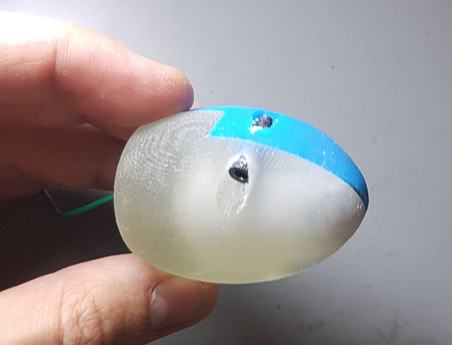
\includegraphics[width=0.3\textwidth]{media/V1_3.png}
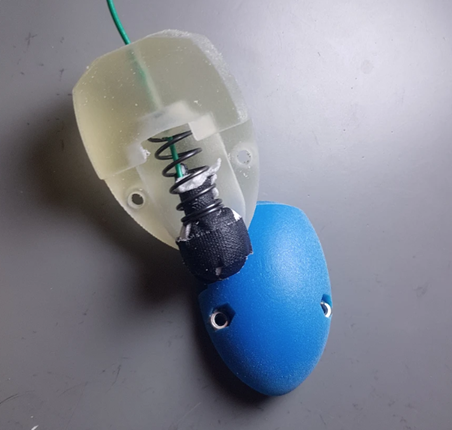
\includegraphics[width=0.3\textwidth]{media/V1_4.png}
   \caption{\label{v1img}  Pictures of both the outside and the inner workings of the first connector prototype}
\end{figure}

% Modular ROBOT LINK EVOLUTION
\begin{figure}
\centering
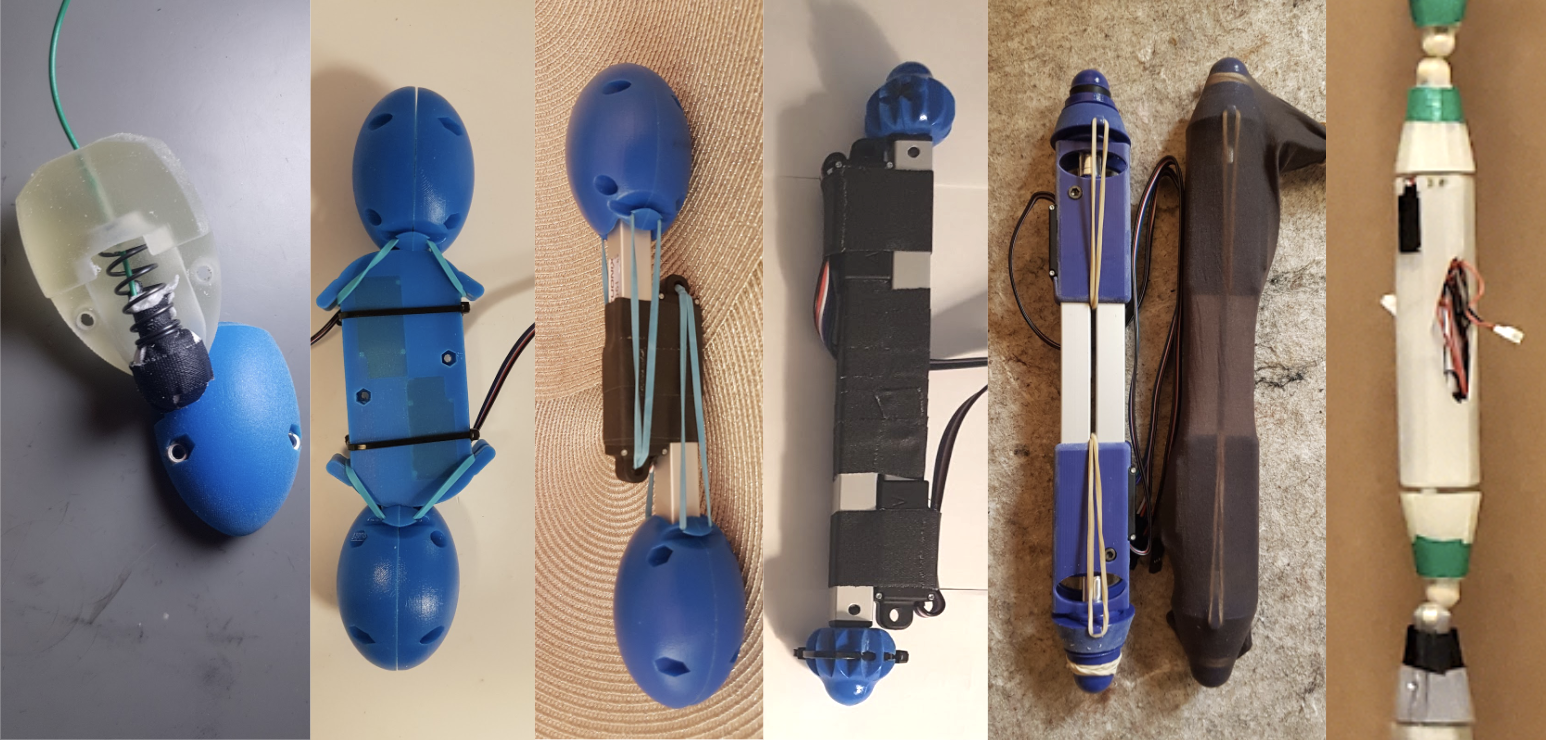
\includegraphics[width=0.45\textwidth]{media/RobotEvolution.png}
   \caption{\label{evolution} The design evolution from the initial manually actuated connector to our most recent design: from oldest to newest from left to right. The current link design is the first iteration that can be entirely printed on a standard FDM 3D printer.}
\end{figure}

% WIRING DIAGRAM
\begin{figure}
\centering
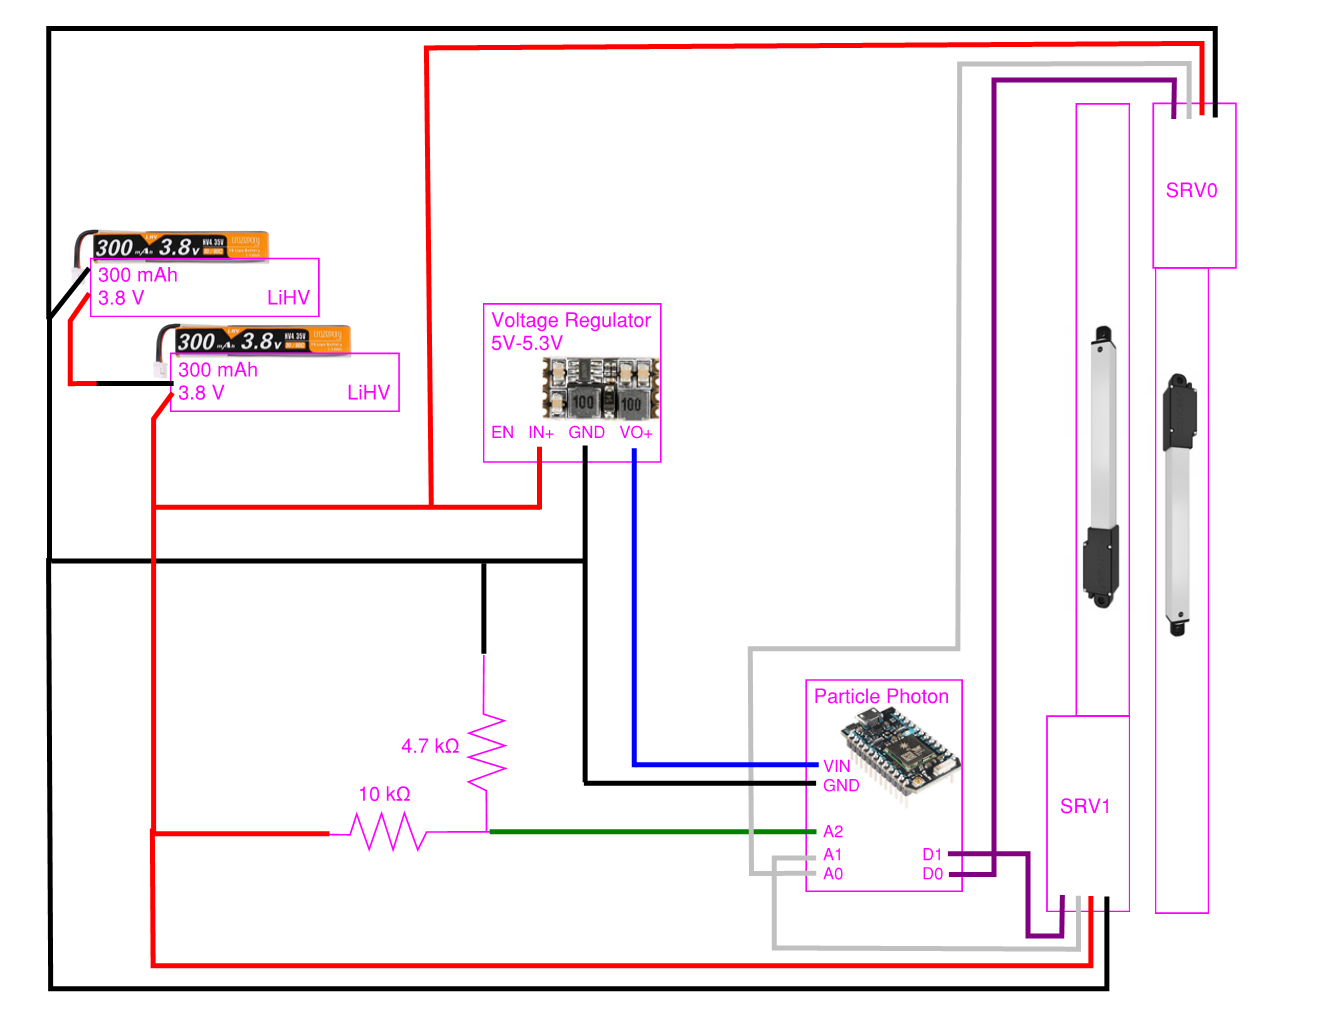
\includegraphics[width=0.45\textwidth]{media/DetailWiringDiagram.png}
   \caption{\label{wiring} An overview of the circuit components and their connections. The actuators are directly powered off of a 7.2V 2S LiPo battery, while the battery voltage is stepped down to 5V for the Particle Photon.}
\end{figure}

Current Link Specifications (Version 4.0):
\begin{itemize}
\item Max-Length: 420mm
\item Min-Length: 270mm
\item Expansion (travel): 150mm
\item Expansion ratio: +55\% 
\item Total Weight: 300g
\item Magnet Diameter: 1/2 inch
\item Max Connection Load: +1.4kg
\item Actuator: 2x Actuonix L-12I, 100mm stroke-length, gear ratio 210:1
\end{itemize}


\subsubsection{Spring Reset Connector}

% OPEN Connector prototype
 \begin{figure}
\centering
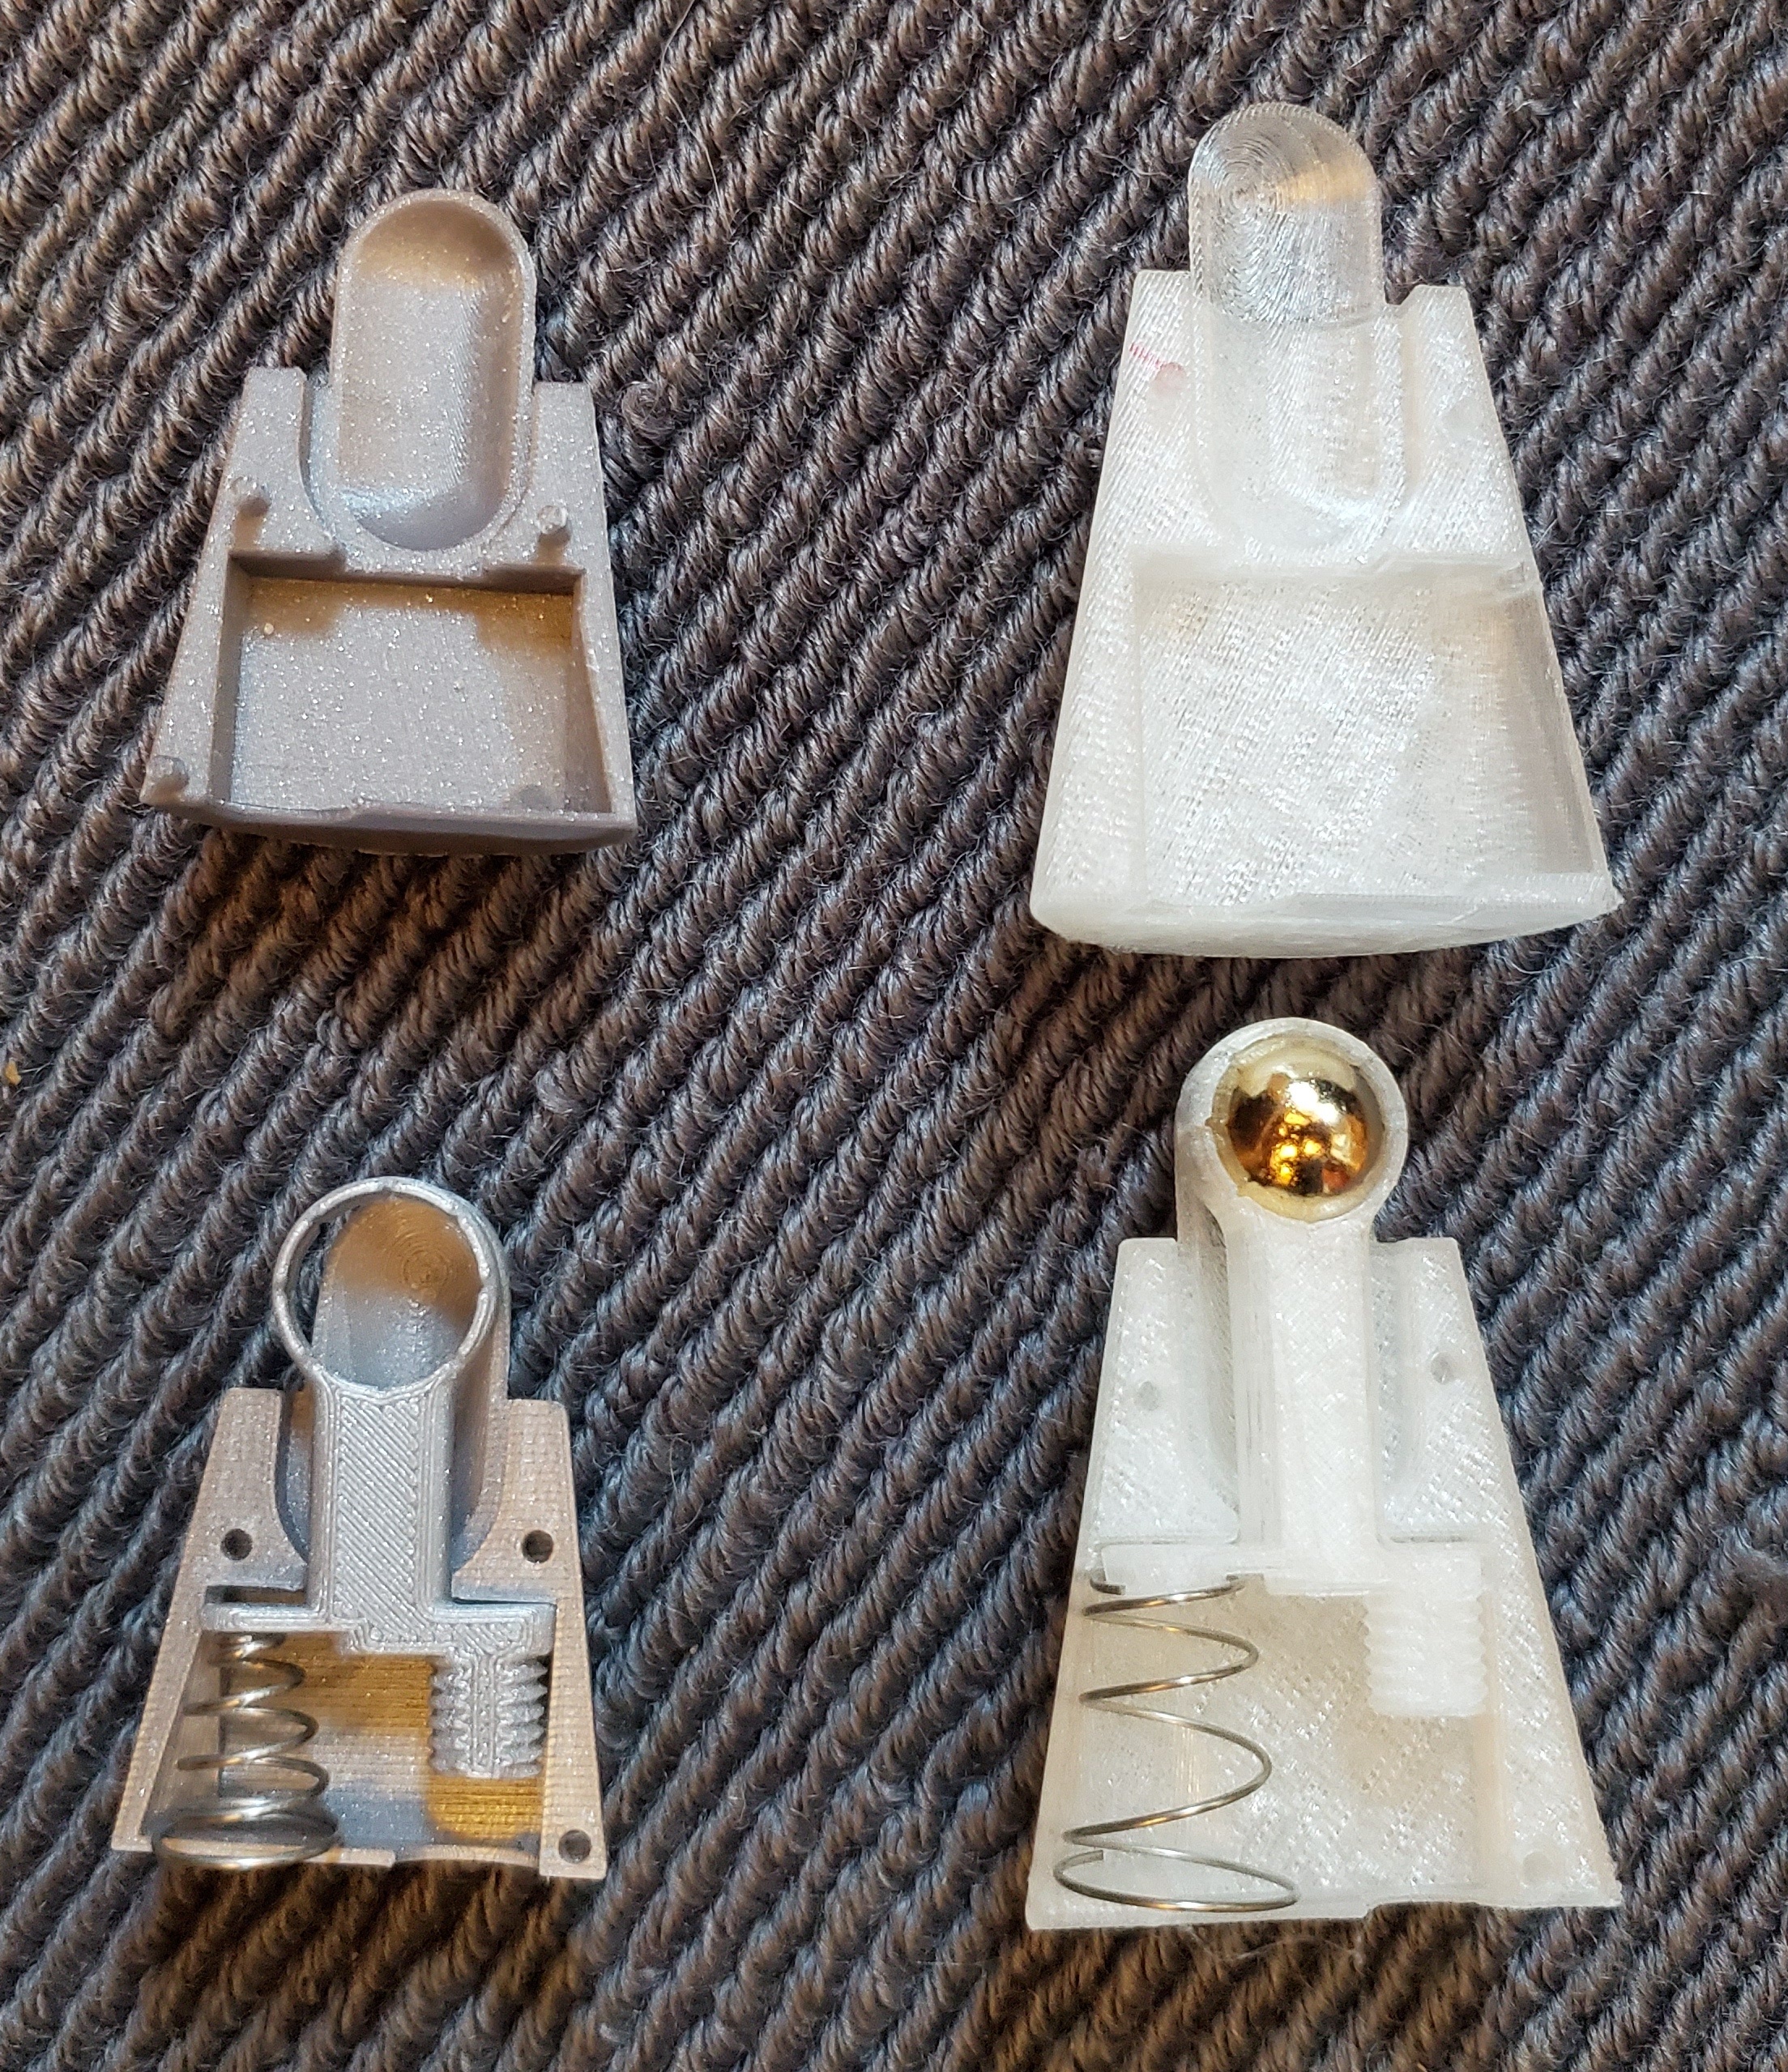
\includegraphics[width=0.4\textwidth]{media/openConnectorPrototype.jpg}
   \caption{\label{openConnector}  We increased the stroke length of our connector from 0.6" (gray) to 0.75" (white) in order to increase detachment reliability.}
\end{figure}

Our previous link design relied on rubber bands to ensure that the magnet sphere would slide back into the tip of the connector in order to re-connect to another link after a detachment. To streamline the design and avoid entangling or breaking of exposed rubber bands, we opted for a connector internal reset spring. The complete assembly including reset spring can be seen in Fig. \ref{openConnector}.

\subsubsection{Achieving Link Symmetry}
% PICTURE OF CONNECTOR OFFSET/MAGNET HOLDER OR Open Connector (new design)
\begin{figure}
\centering
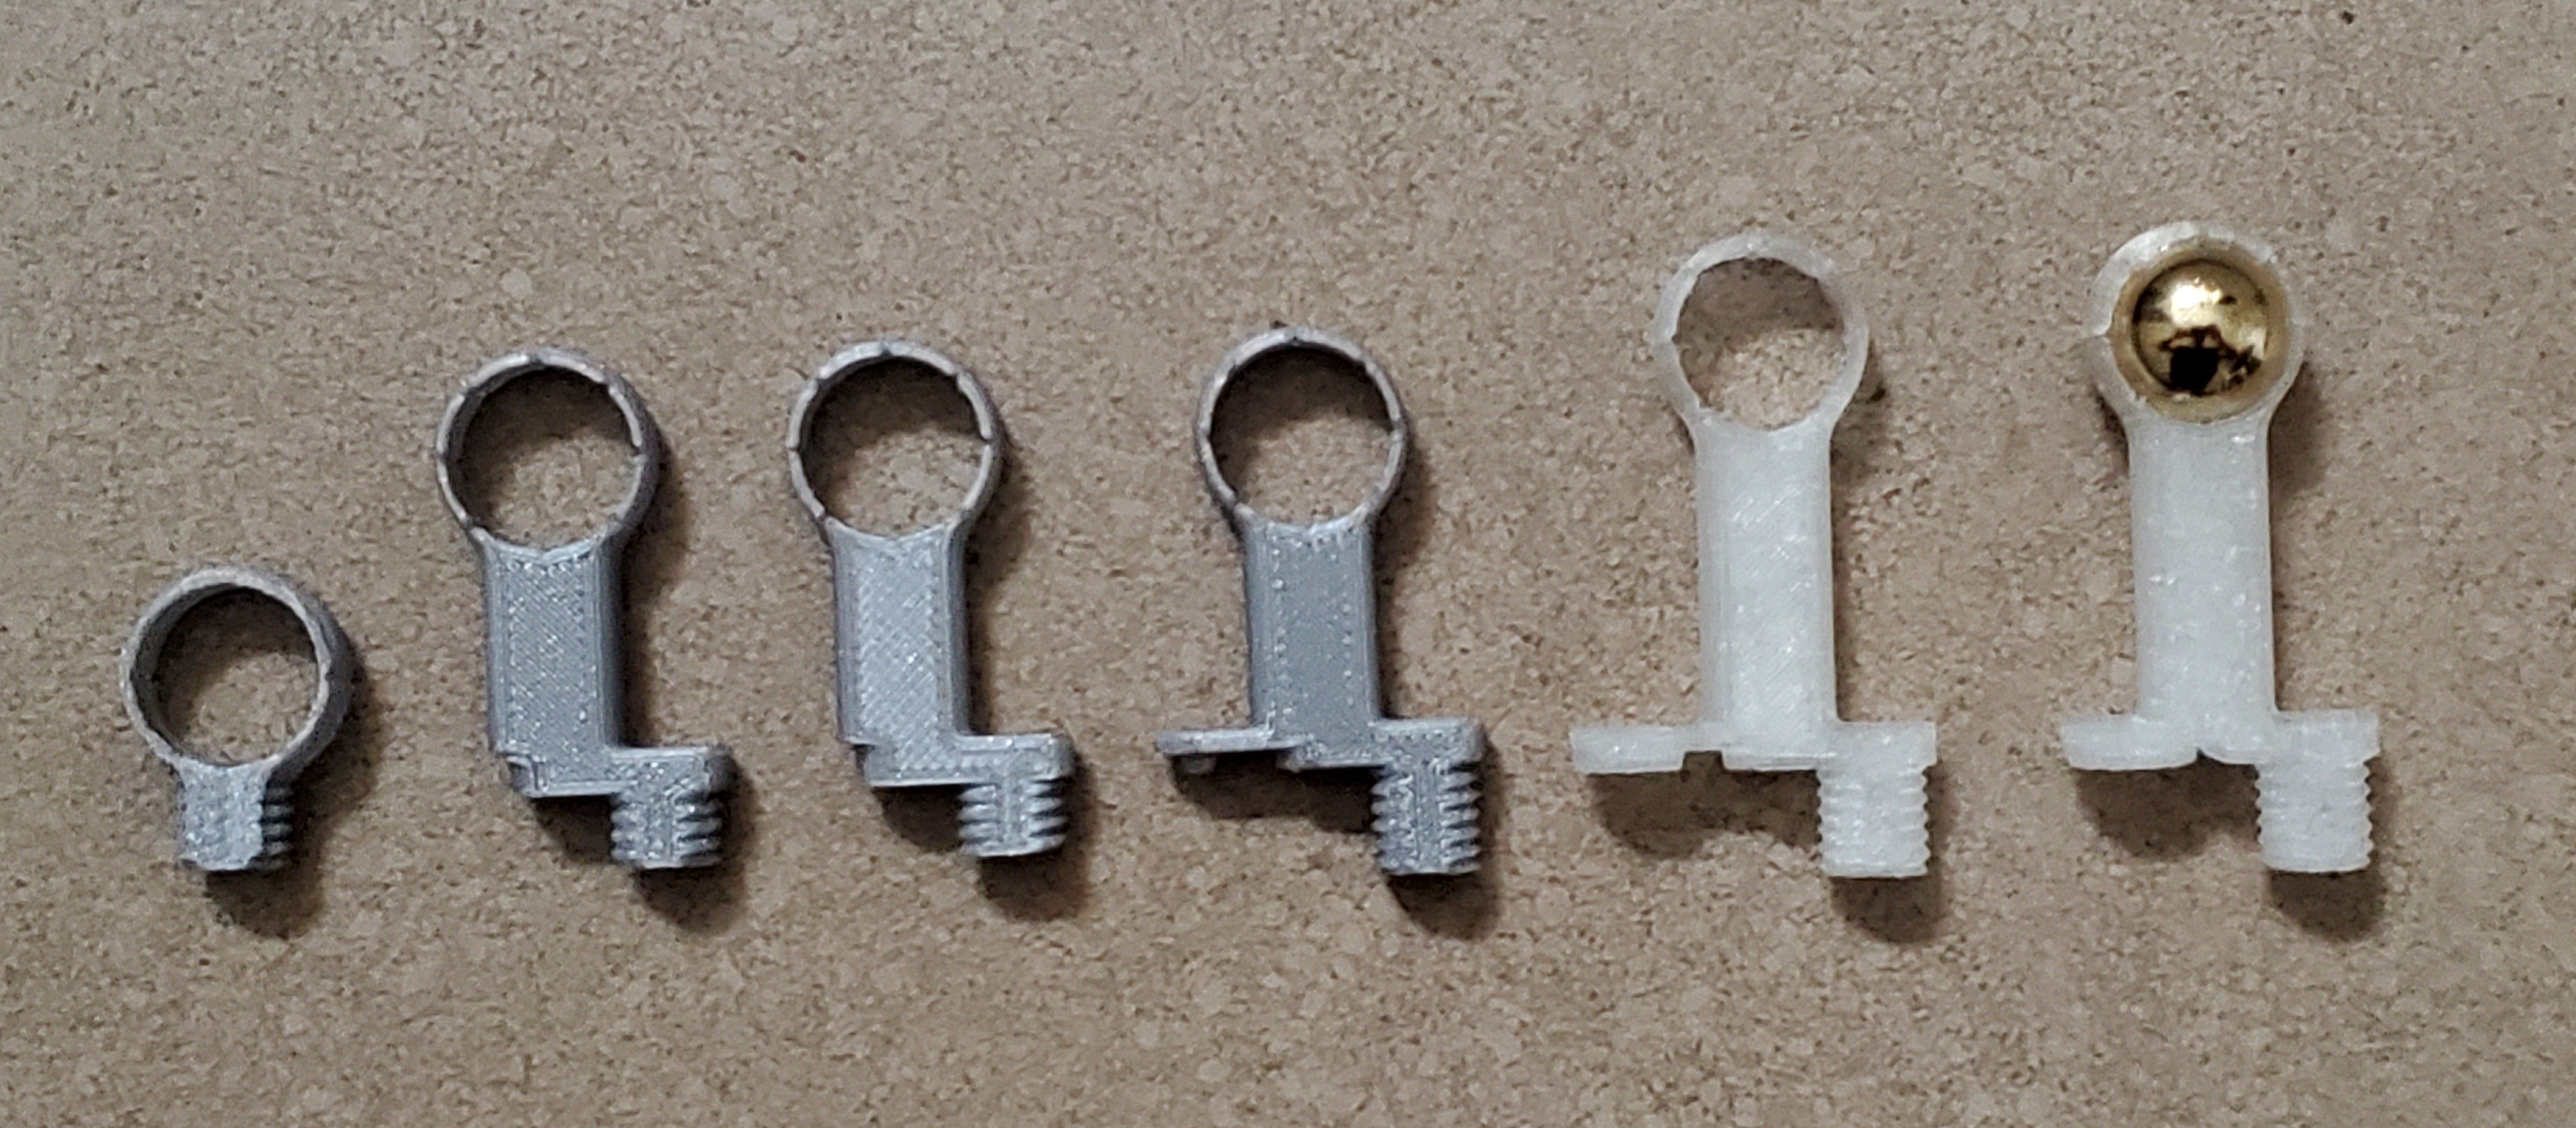
\includegraphics[width=0.45\textwidth]{media/MagnetHolder_Evolution.jpg}
   \caption{\label{MagnetHolderEvolution} The evolution of our FDM 3D printable magnet holders from oldest to newest from left to right respectively. The current magnet holder design of our $\frac{3}{4}$ inch retraction length connector with a spring based reset mechanism is the model on the very right.}
\end{figure}

To minimize the minimum length of each link, the two prismatic actuators sit side by side in opposite directions. This leads to an offset in the actuator axis of motion, and therefore in an asymmetric actuation pattern. To make sure the links are symmetric in themselves, we designed the magnet holder to include an offset to center the axis of the connector on both ends of the link as seen in Fig. \ref{MagnetHolderEvolution}.

\subsubsection{Optimizing Expansion Ratio}
We found that Actuonix L12-I actuator with a stroke length of 100mm provides the links with the best expansion ratio, since a smaller percentage of the actuator length is occupied by the motor and internal controller of the actuator. In prior versions we struggled to reach the desired expansion ratio of 41.5 percent, partially due to the use of the smaller 50mm actuators, but also due to the formerly oversized connector design. By decreasing the magnet ball diameter from 5/8" to 1/2" inch and appropriately reducing the connector size, we managed to maximize the expansion ratio to 55\% (see Fig. \ref{v3expansion}).

% EXPANSION RATIO EXAMPLE
\begin{figure}
\centering
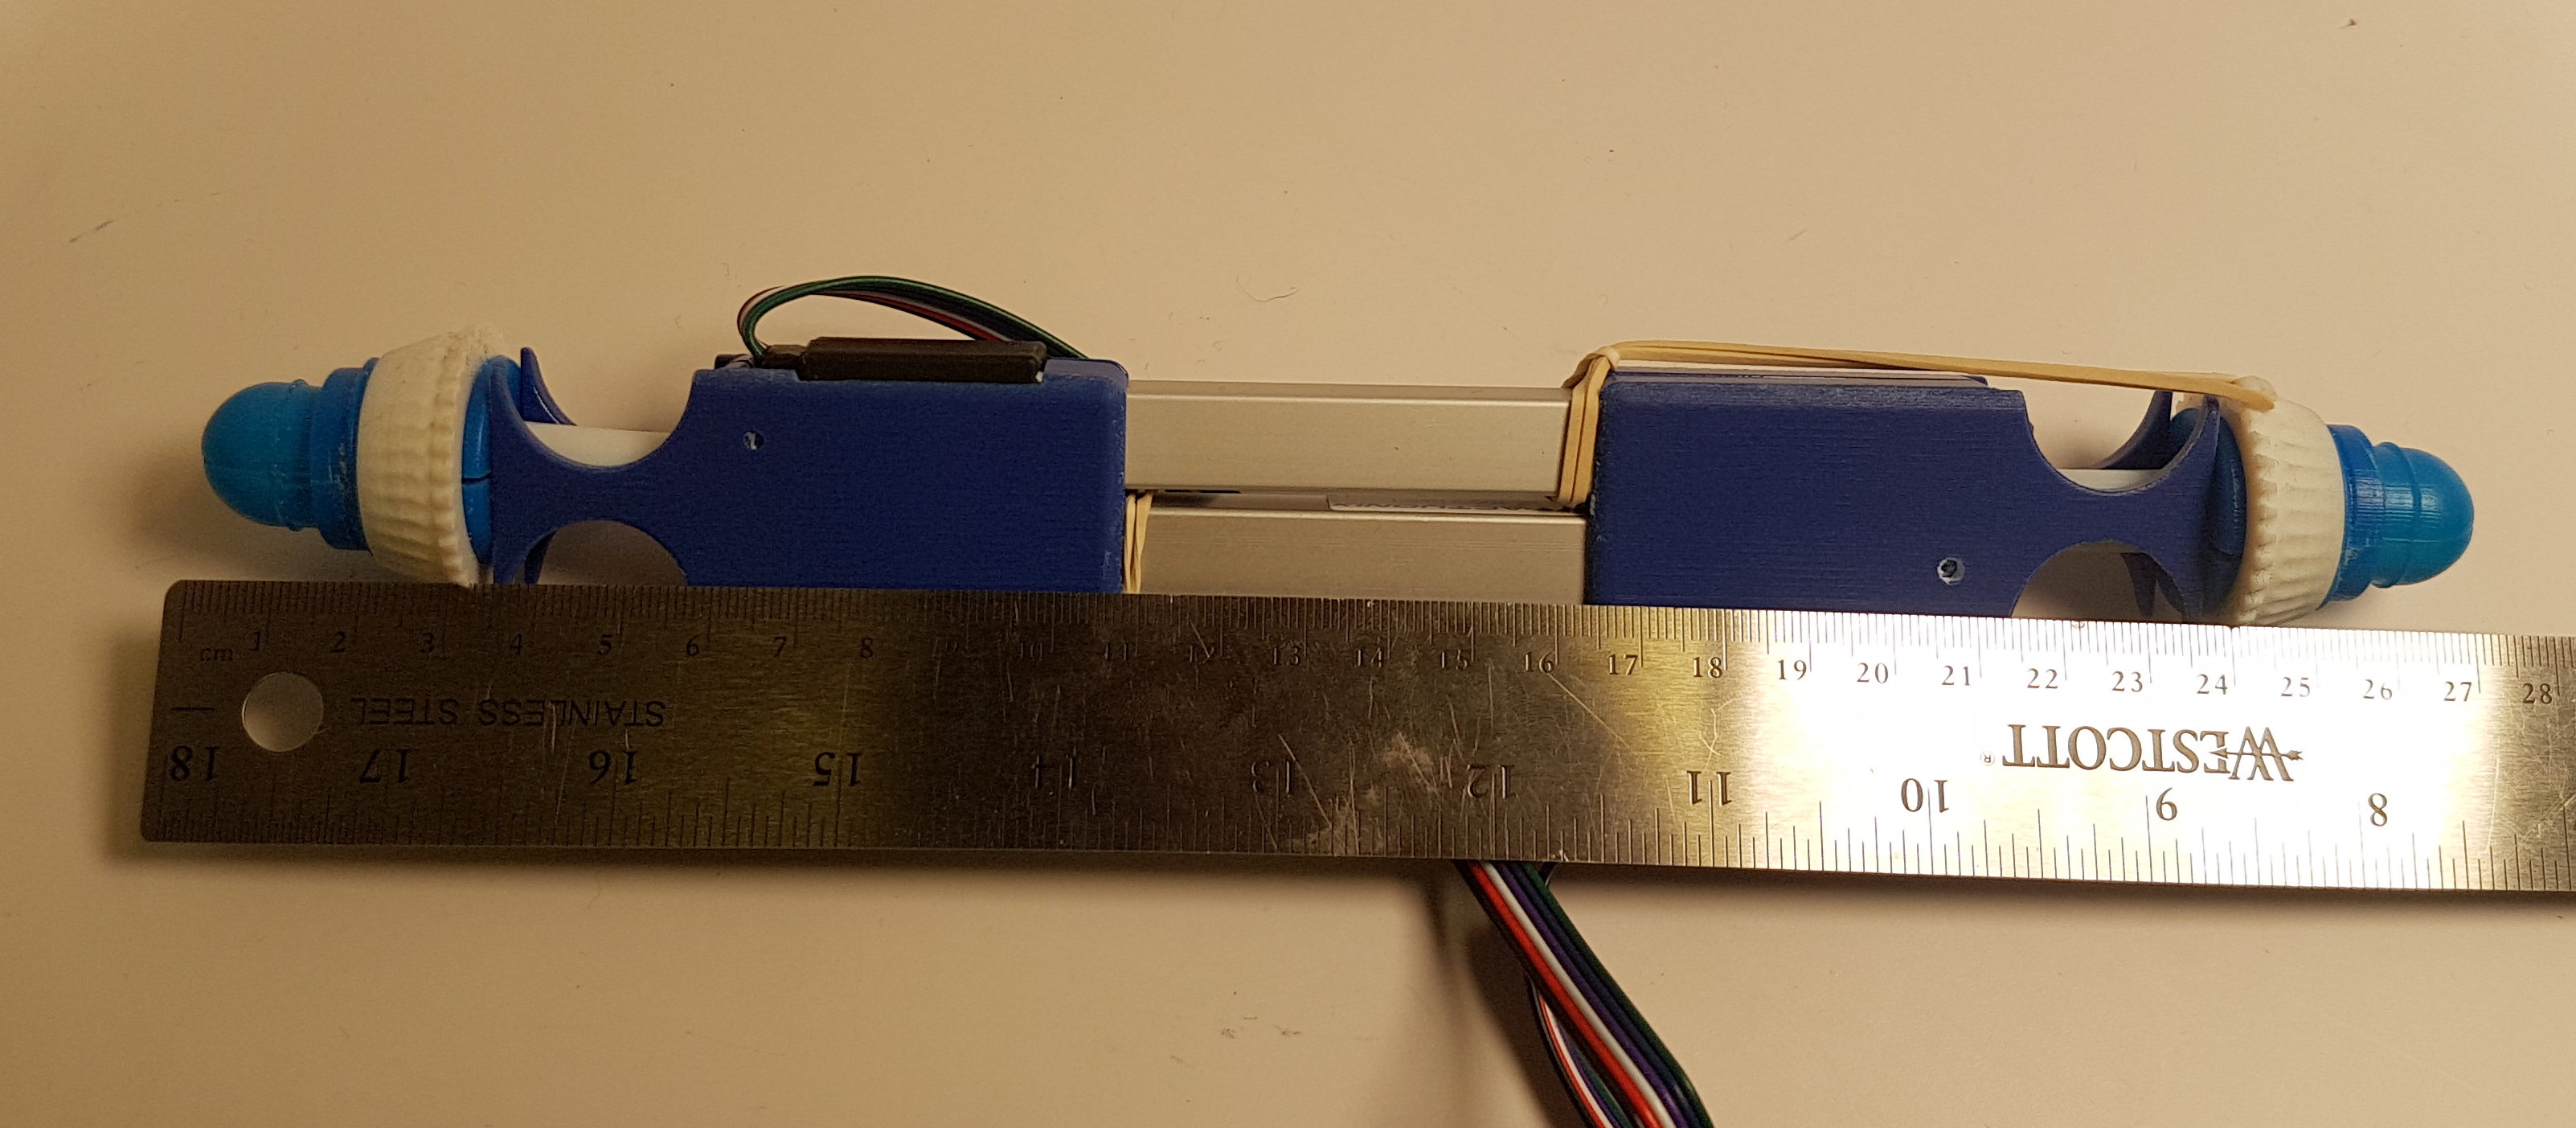
\includegraphics[width=0.45\textwidth]{media/V3_2contracted.jpg}
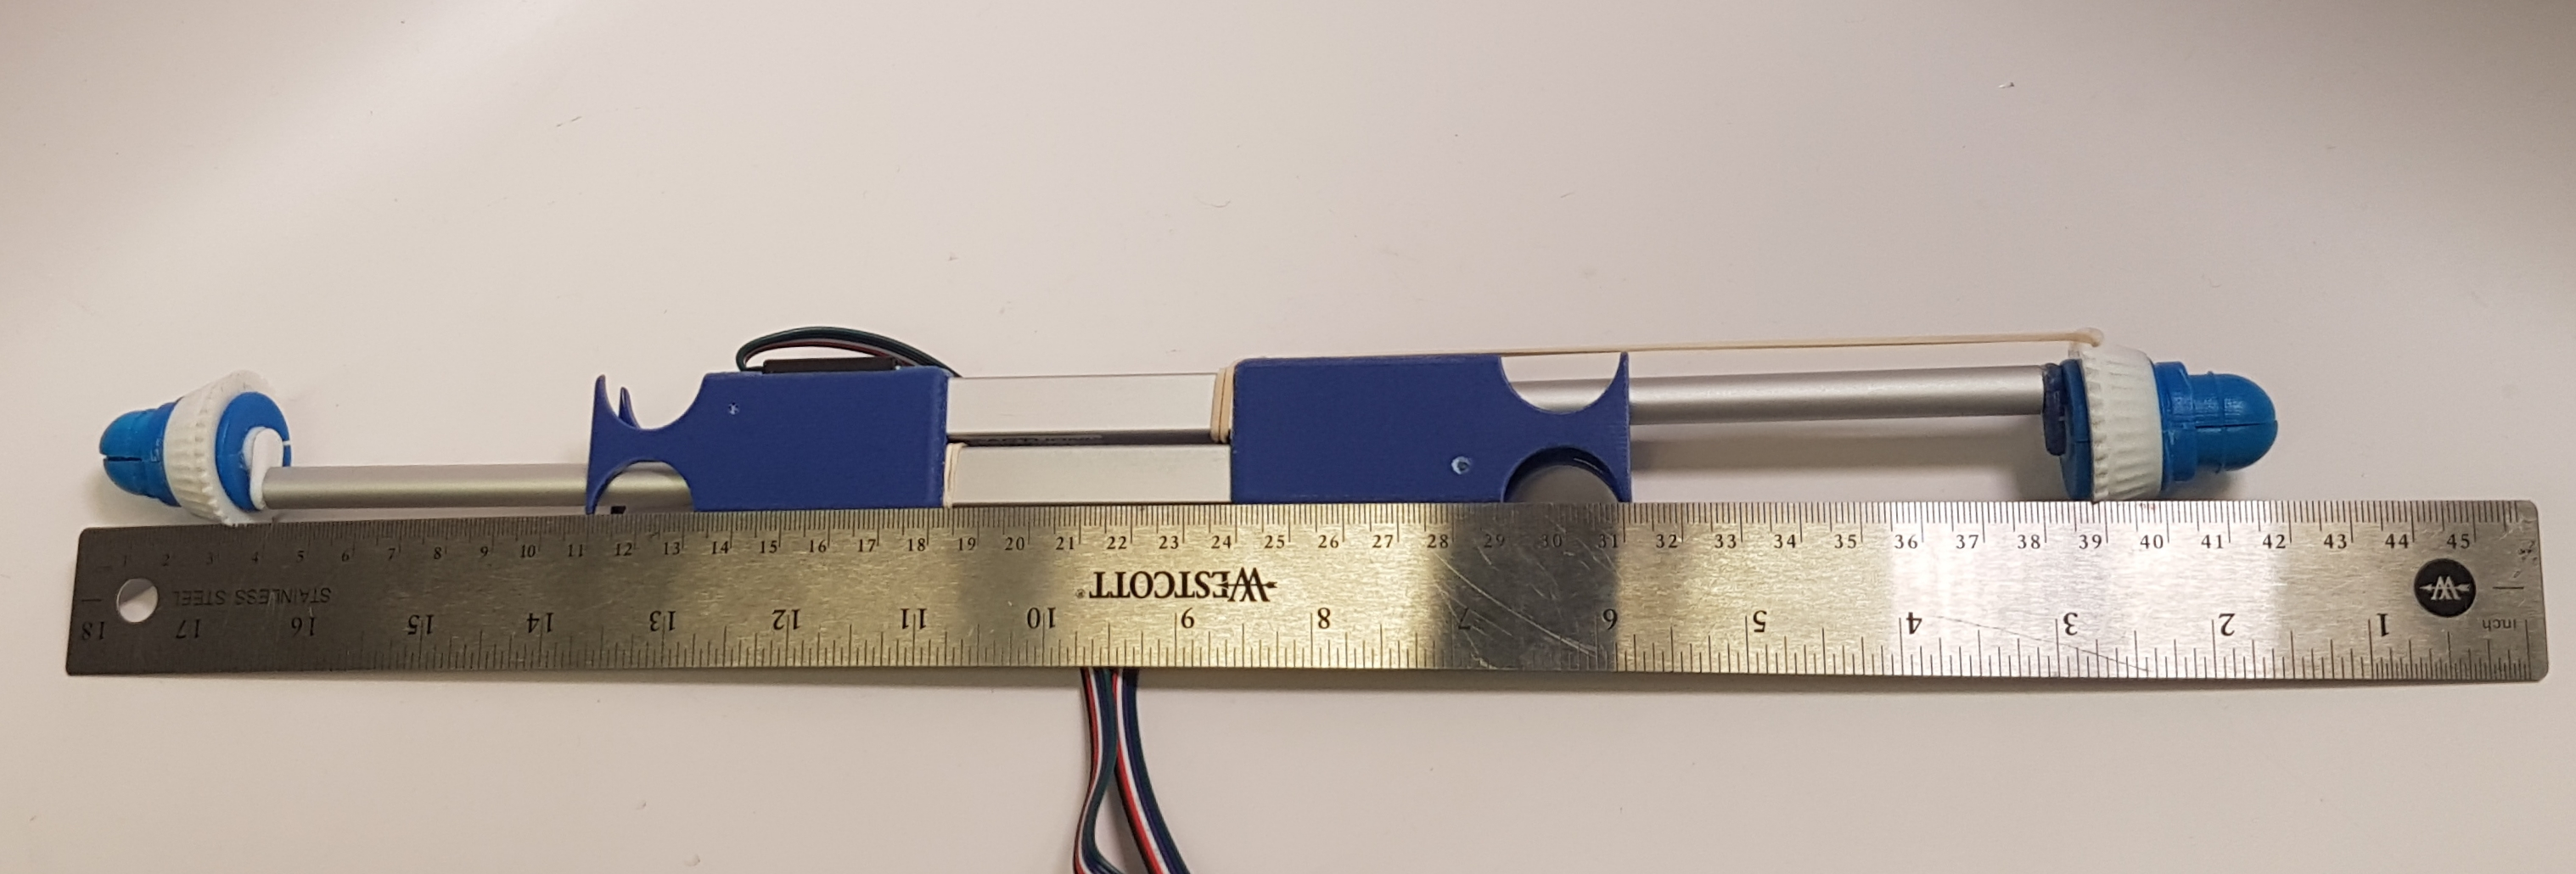
\includegraphics[width=0.45\textwidth]{media/V3_2expanded.jpg}
    \caption{\label{v3expansion}An older Link version Expanded and Contracted for scale comparison. The expansion ratio of the link is a crucial design parameter for achieving a toppling tetrahedron motion.}
\end{figure}

\subsubsection{Optimizing the Attachment/Detachment Geometry}
% Connector Ridge Detachment Diagram
\begin{figure}
\centering
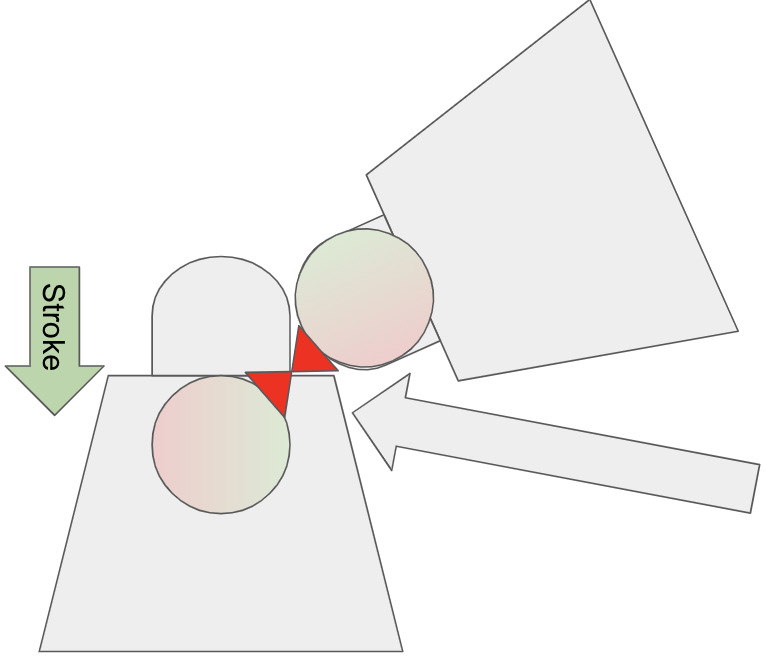
\includegraphics[width=0.4\textwidth]{media/ConnectorRidge.png}
   \caption{\label{fig_connectorRidge} The connector ridge prevents connected links from sliding along the connector during the magnet retraction process. The thereby attained distance between the magnet spheres is the key to detaching the links from each other.}
\end{figure}

The connector design must ensure that during the retraction motion the attached link doesn't follow the magnet and hence fails to detach. Simultaneously, the links have to be able to attach to each other at angles as small as 30 degrees, thus simply increasing the size of the connector on the sides is not an option. This problem was solved by adding a ridge to stop a connected link from following the magnet during the retraction phase\ref{fig_connectorRidge}.

\subsubsection{Preventing Connector Shattering}
During the connector design, we struggled with the connectors shattering on impact with another connector\ref{shatter}. Earlier versions of the Robot Metabolism links were 3D printed on the Stratasys J750, the connectors were either to brittle if printed without Tango+ or too soft if printed with a small percentage of Tango+. We encountered the seam issue when SLA printing the connector with the Formlabs Tough Resin. The old link design was exposing the gap where the two connector shells meet--the weakest section of the connector--to the most impact. We both redesigned the connectors to have a connector tip without seams, and 3D printed it in SLS Nylon for resilience. We needed to increase the thickness of our shell to comply with SLS printing requirements and had to send the parts out to be manufactured off site, thereby reducing our flexibility in the prototyping process. This lead us to abandon our initial design entirely, and move to an FDM printed robot link design. PLA's impact resistance has solved our connector shattering problems in our most recent tests.

\begin{figure}
\centering
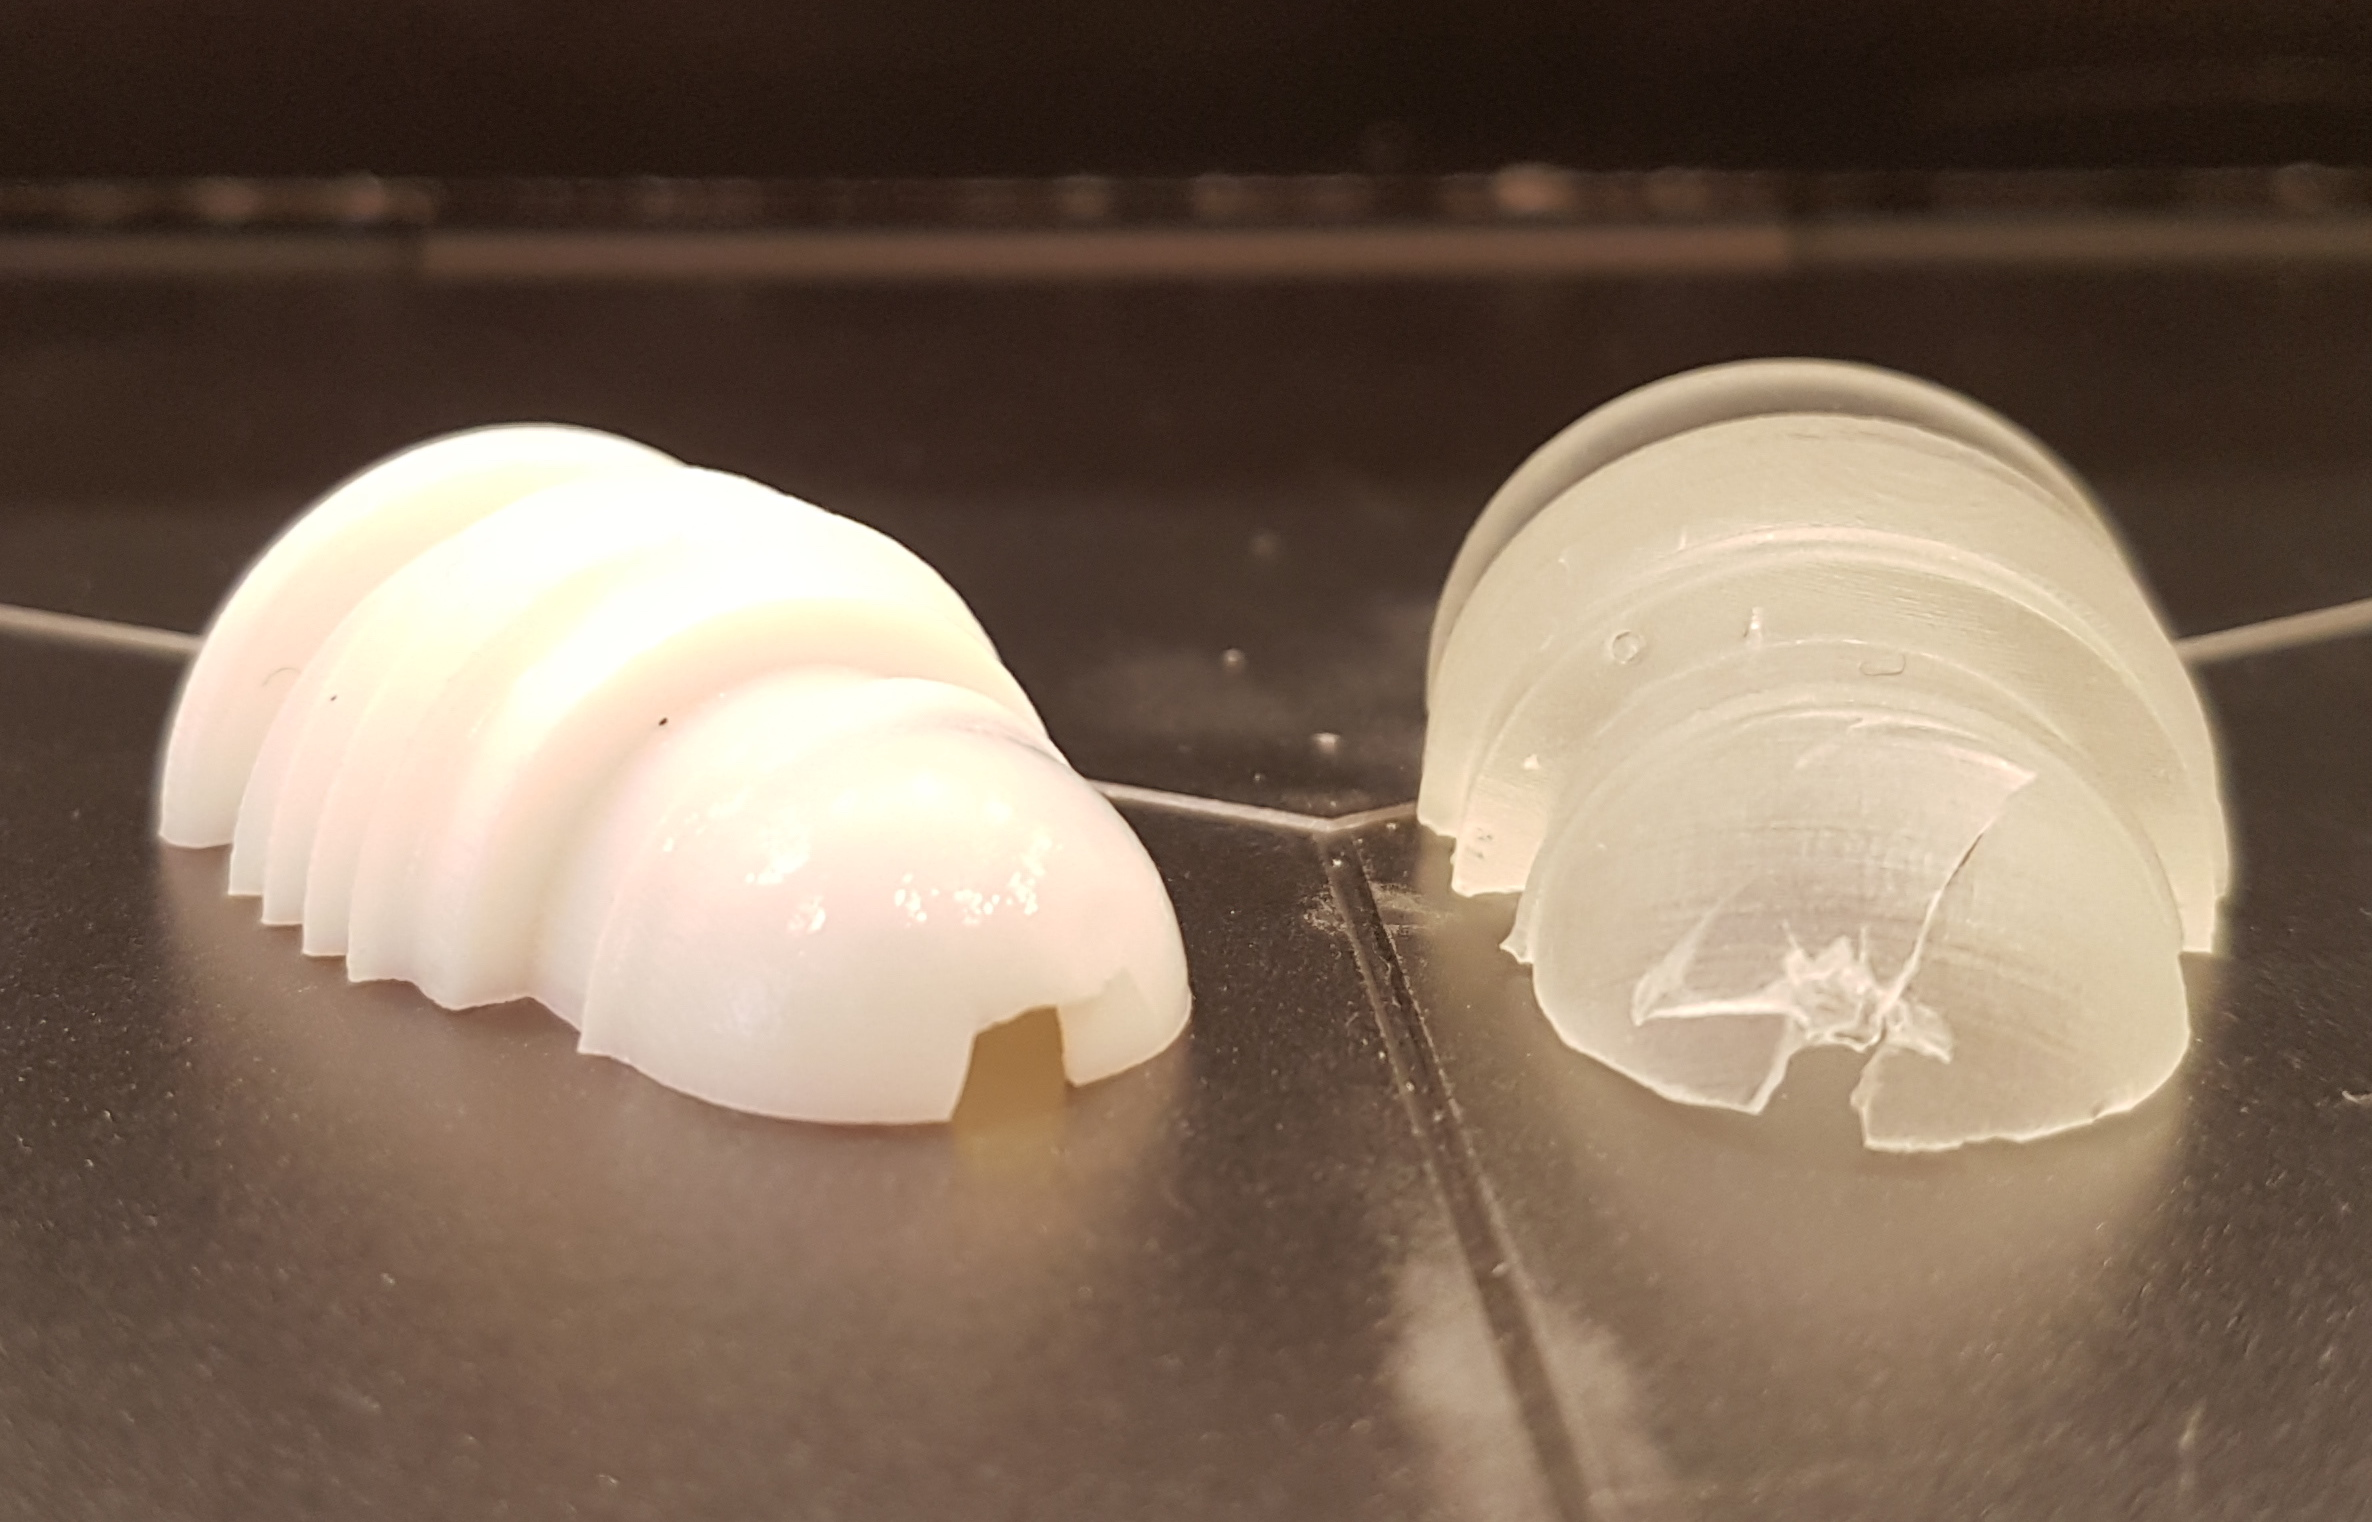
\includegraphics[width=0.45\textwidth]{media/shatter.jpg}
   \caption{\label{shatter}  Shattered connector shells: (left) printed on Stratasys J750 and (right) printed with Formlabs Form2}
\end{figure}

\subsubsection{Streamline Link Wiring} Our previous link versions did not include wire management, and were controlled from a breadboard with a mounted Particle Photon. In our latest design, we included wire channels as seen in Fig. \ref{fig_wireChannel}. The wire channels allow the motor wires to be routed inside the center body shell and prevent any risk of entanglement (see Fig. \ref{fig_linkprototype}).

\begin{figure}
\centering
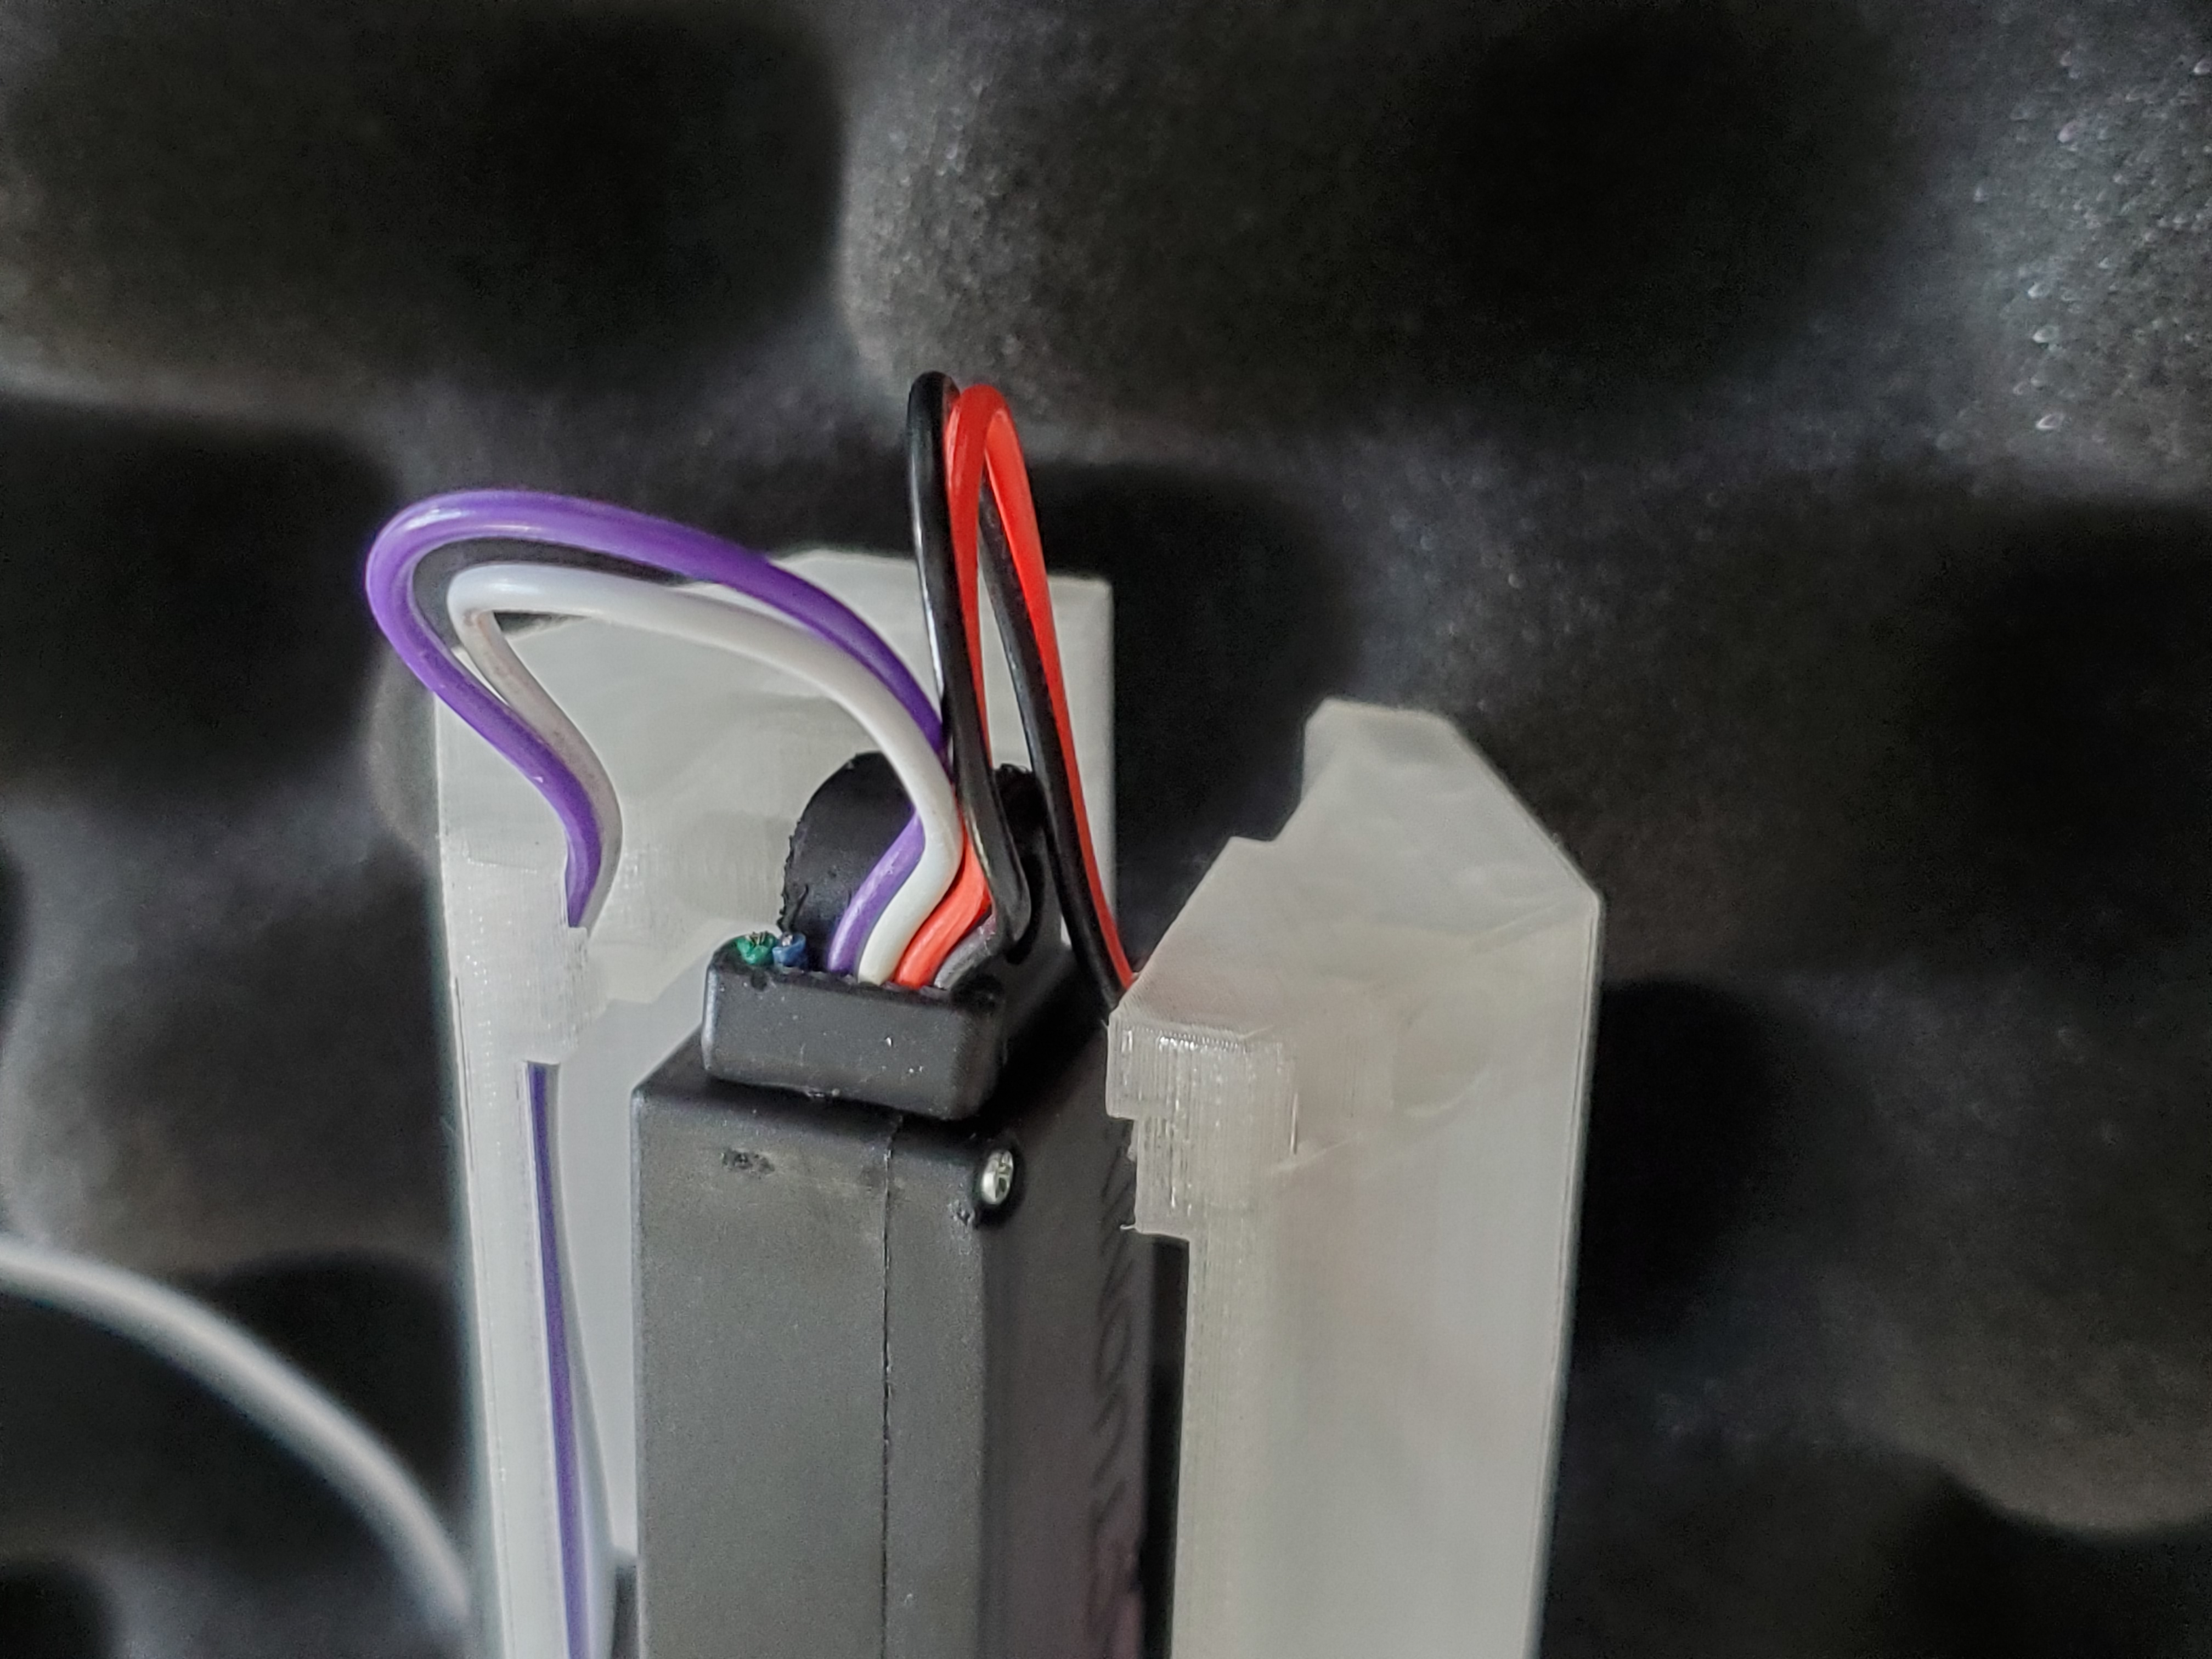
\includegraphics[width=0.45\textwidth]{media/wiringChannels.jpg}
   \caption{\label{fig_wireChannel} This images shows how the wires are routed through the body shell components to the inside. The wires are displayed loosely for demonstration purposes only: when assembled, the robot links do not have any dangling wires.}
\end{figure}

\begin{figure}
\centering
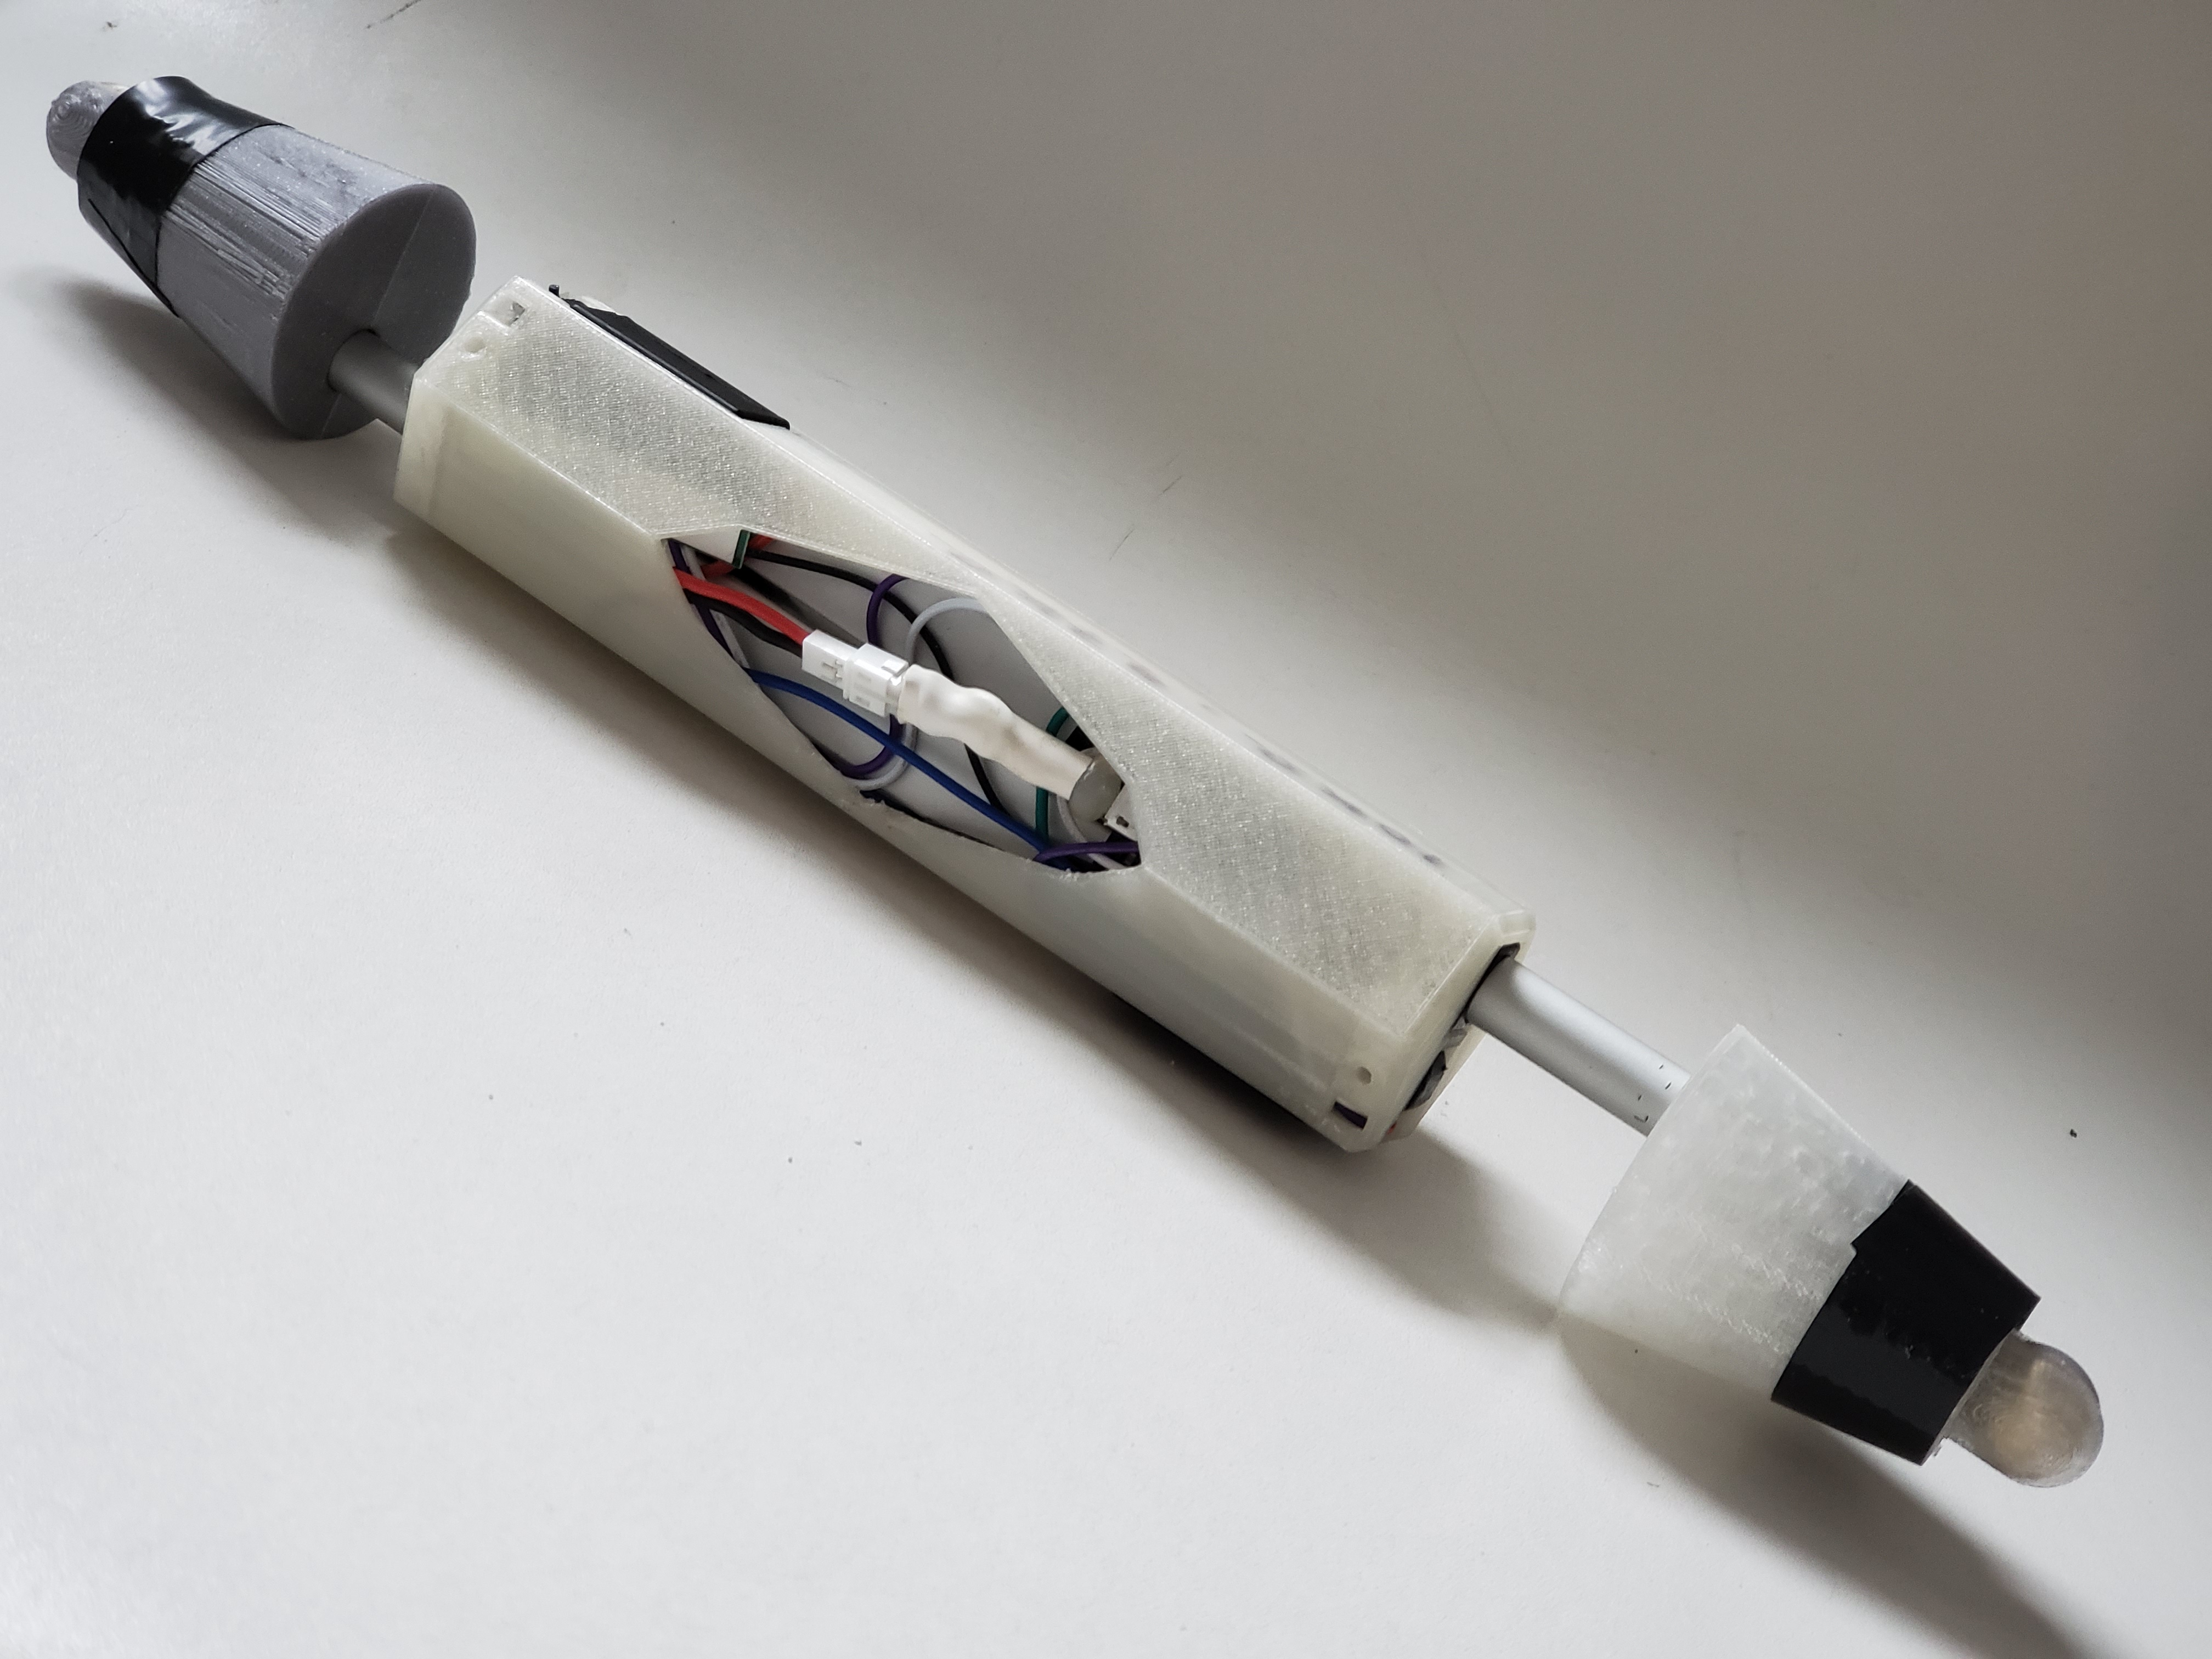
\includegraphics[width=0.45\textwidth]{media/linkprototype.jpg}
   \caption{\label{fig_linkprototype} Assembled link prototype shows that all wires are housed inside the shell.}
\end{figure}

\subsection{Micro-Locomotion: Single Link Crawl}
In an effort to explore the capacity for locomotion of single links, we found that when individually actuating each linear actuator, we can reproduce an inch-worm crawl. This provides each link the capacity to move itself linearly across a surface. Since we are not trying to solve the question of origin i.e. we start our exploration from a basic assembled structure such as a triangle or a tetrahedron, this finding is pleasant but not necessary for the success of this project.

\section{Software}
The main challenge in controlling numerous autonomous robot Links is developing a Software Infrastructure for communication and coordination. For this project, a centralized approach, using a Server-Client model, was implemented.

\begin{figure}[H]
\centering
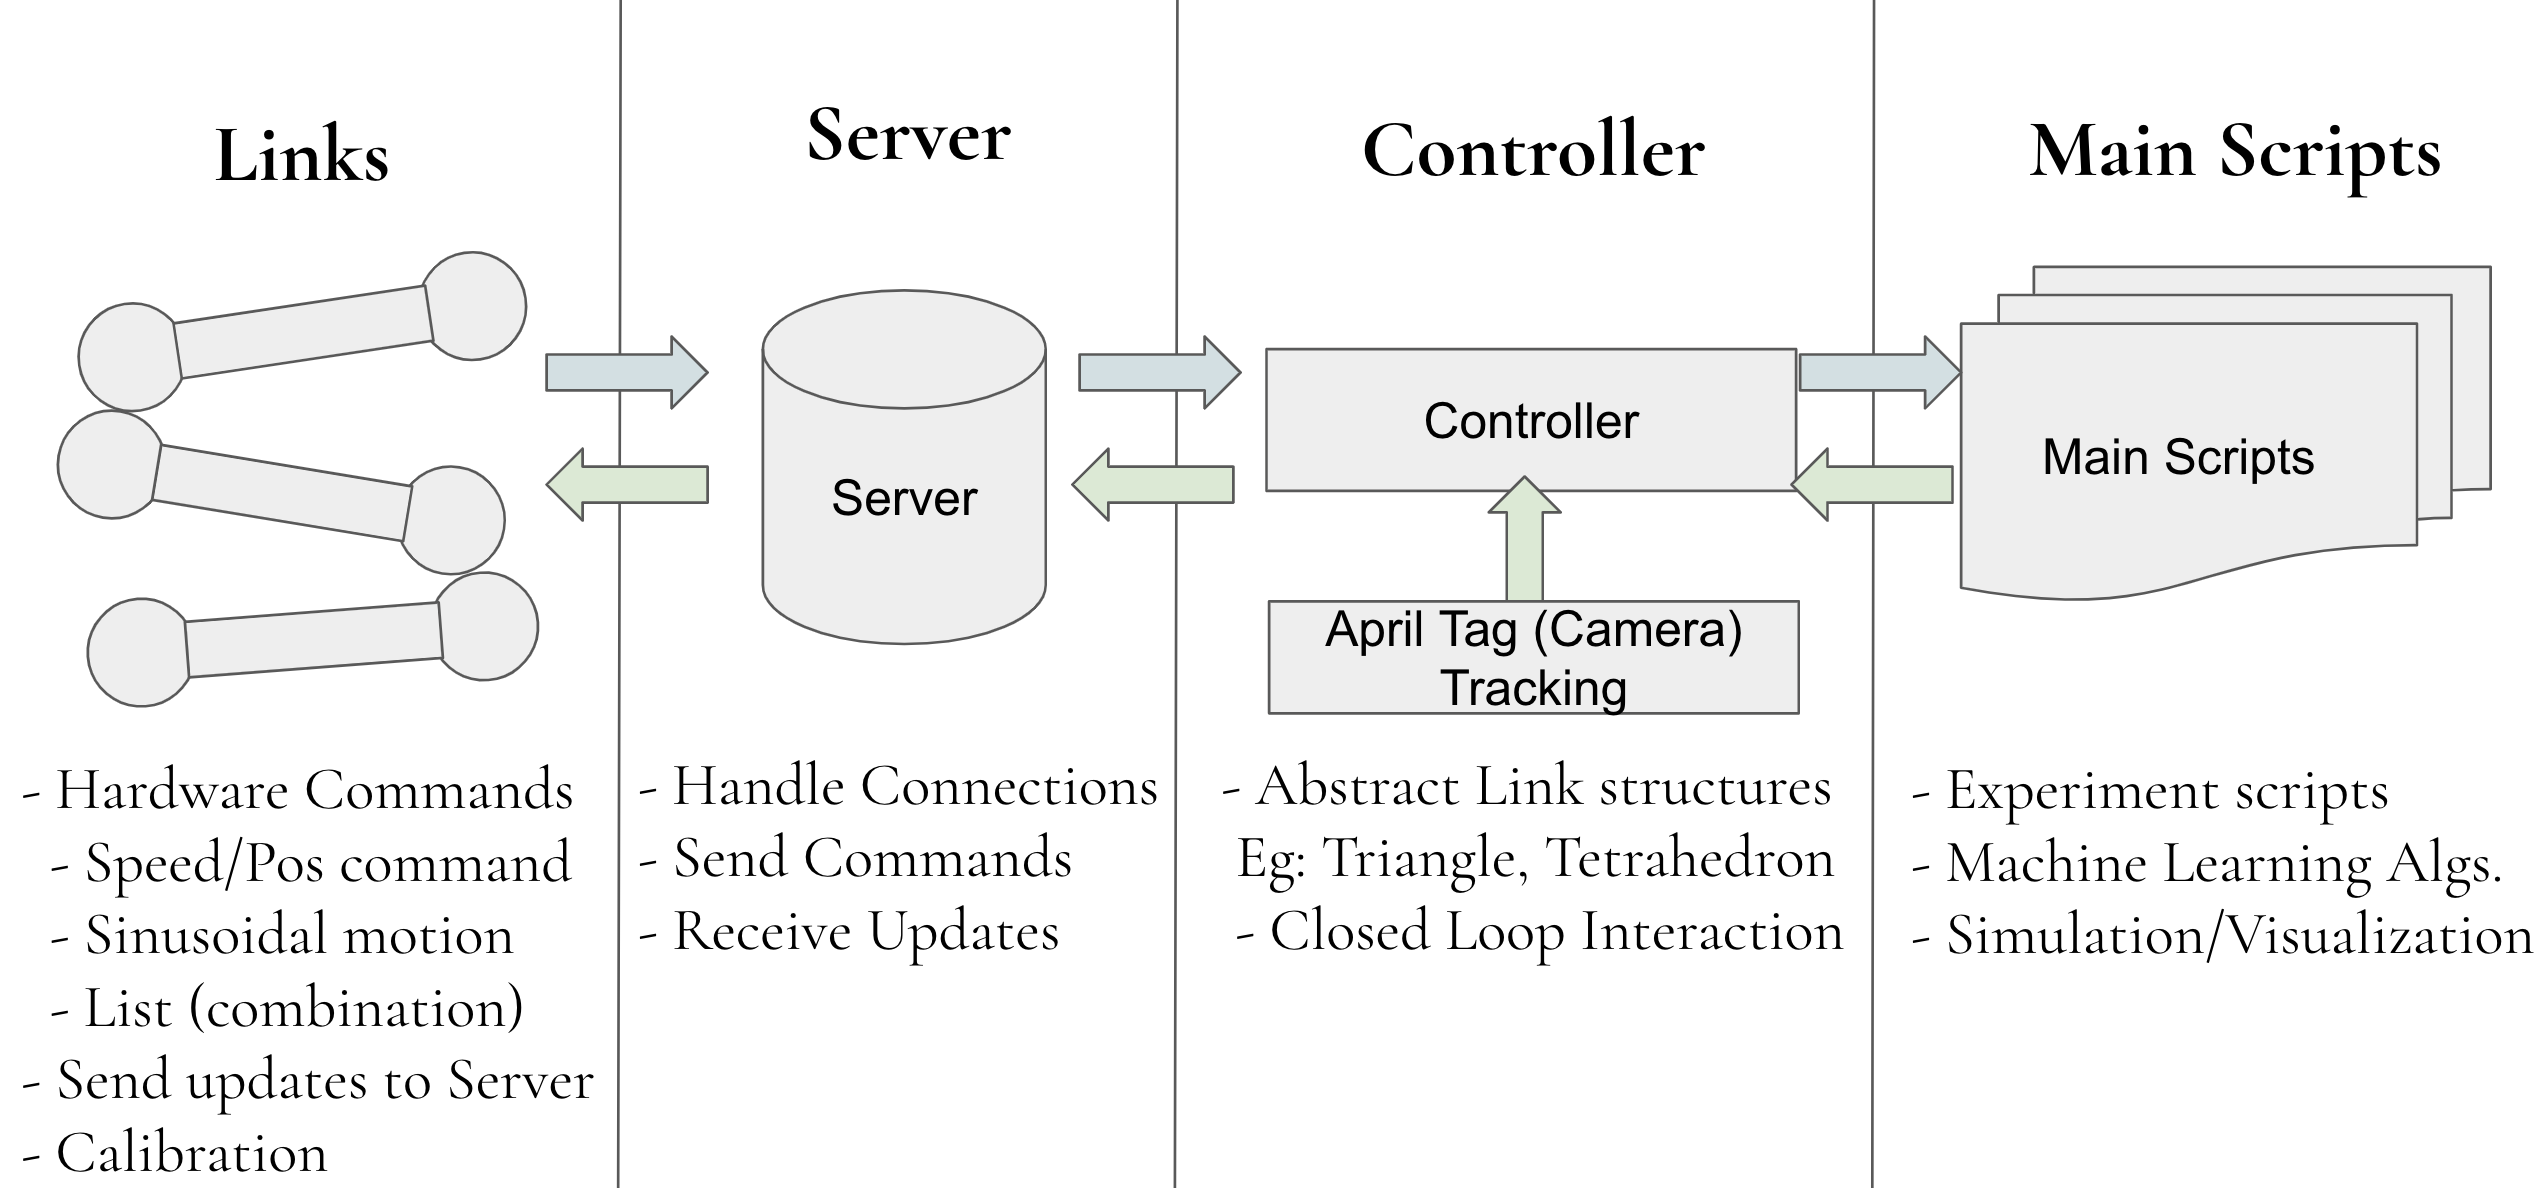
\includegraphics[width=0.485\textwidth]{media/SoftwareInfrastructure.png}
   \caption{\label{fig_softwareInfrastructure} Software Infrastructure can be broken into 4 distinct parts. All parts closely interact with one-another to allow closed-loop control.}
\end{figure}

Every Link connects to a common WiFi network via the on-board Particle Photon, acting as individual clients. Subsequently, they use Socket API to connect to a central Device - eg. a laptop - which runs the Server scripts. On the Server, "Controller" scripts then interface and coordinate the Links' actions based on information from a Camera and each Link, in a Closed Loop, for the "Main" Scripts (which run experiments). Fig. \ref{fig_softwareInfrastructure} gives a graphic description of the 4 parts of this system.

\subsection{RML Protocol}

Since the Particle Photon runs C++, and all Server-side Scripts run Python, a common "language" and protocol needed to be established for socket communication. Hence, the \textit{RML Protocol} is used.

The RML Protocol uses Packages consisting of C++ structs and datatypes. An RMLP Package consists of 3 parts:

\subsubsection{Header} The header contains two bytes, one holding the Package Type and the other the Package Length. This allows the program receiving the package to know how many bytes to read, and how to interpret them based on package type.
\subsubsection{Body} The body varies based on the type of package. Optimizations were made to minimize the sizes of all types of packages. The body is usually on the order of 5 bytes, making for very efficient data transmission, even at high frequencies.
\subsubsection{Footer} The footer contains a 16-bit CRC-15 checksum of the package\cite{CRC_Ross}. CRC-15 was picked due to its concise and efficient implementation that can easily run on the Photon. Packages with incorrect checksums can be ignored by the receiver.
\\
These 3 parts are appended to create a complete RMLP Package, as illustrated in Fig. \ref{fig_packageFormat}

\begin{figure}[H]
\centering
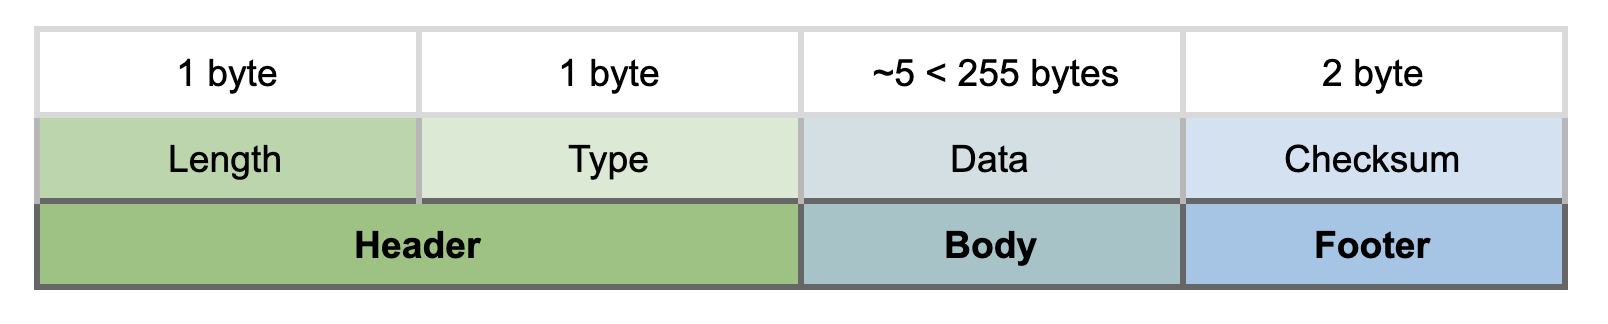
\includegraphics[width=0.485\textwidth]{media/PackageFormat.png}
   \caption{\label{fig_packageFormat} 3 parts - Header, Body, Footer - appended to form RMLP Package}
\end{figure}

\noindent Take, for example, the Update Package, in C++ syntax:

\begin{lstlisting}[language=Python]
union MSG_update{
    struct MSG_UPDATE_DATA{
        char device_status;
        unsigned char srv0_pos;
        unsigned char srv1_pos;
        unsigned char srv0_raw;
        unsigned char srv1_raw;
        unsigned char bat_status;
        unsigned char srv0_vel;
        unsigned char srv1_vel;
        unsigned short prev_checksum;
    } get;
    uint8_t bytes[MSG_UPDATE_LENGTH];
} msg_update;
\end{lstlisting}

The use of a union allows reading and writing the data as individual bytes and as other int datatypes like "char" and "short" interchangeably. In order to reduce the size of the package, data is expressed using the lowest possible number of bytes. Hence, most data is expressed using 1-byte chars. The update package in the example above is sent periodically by the Link to the Server with hardware information and the Link's status. It is ensured that the update is only sent once every 10 seconds, unless there is a change in robot status, to minimize network traffic.

Similarly, numerous package types have been implemented and optimized to facilitate communication. These can be found under RMLProtocol.h in the code repository.
\\
\subsection{Server}

To run experiments with potentially hundreds of Links, it was necessary to run an efficient server. Due to Python's offerings in simplicity, convenience, and libraries, it was decided that the Server would be implemented in Python.

The Server-Client Model requires that the Server accepts connections from and handles multiple clients simultaneously. Hence, the Server uses a multi-threaded approach - wherein a Listening Thread accepts new socket connections from Links, and each Link is then associated with a new "LinkHandler" Thread on the Server. 
\\
\subsubsection{Listening Thread}
The Listening Thread runs uninterruptedly after the server's conception, and constantly listens for new Link Connections. The UNIX timestamp corresponding to the start time of this thread is stored, and is subsequently used as "Time 0" by all Links, enabling all devices to use a synced clock. Every time a connection from a link is accepted, a new LinkHandler Thread begins, and the Listening Thread waits for the next Link to connect once more. A lookup table holds all the initiated LinkHandler threads so that Controller Scripts can use them to communicate with Links.
\\
\subsubsection{LinkHandler Thread}
The LinkHandler Thread is responsible for all communications with a Link after the initial socket is connected by the Listener Thread. It executes the following process:

\begin{enumerate}
    \item Receive "Hello Package" containing Link's Device ID
    \item Send "Time Epoch package" which holds the start time UNIX timestamp in it
    \item Enter Update loop:
    \begin{enumerate}
        \item Receive Update package via TCP connection and verify CRC-15 checksum
        \item Update local Link values from package
        \item If socket disconnects or no update received in 10 seconds, exit loop, or else, repeat.
    \end{enumerate}
    \item Close socket connection cleanly
    \item End Thread
\end{enumerate}

\noindent The above Thread only uses the socket to receive data. \\\\ At the same time, the Controller Thread uses the socket only to send command data as follows:

\begin{enumerate}
    \item Encode commands into bytes using RMLProtocol (example: Sinusoidal command)
    \item Enter Checksum loop:
    \begin{enumerate}
        \item Write package to Link over TCP connection
        \item Wait for Update package to be received asynchronously by the LinkHandler Thread.
        \item If checksum indicates command was received without corruption, the loop is exited, or else loop repeats.
    \end{enumerate}
\end{enumerate}

On the Server, the Controller can send commands to the Link (instantly) in the Main thread while the LinkHandler receives update packages asynchronously in an independent Thread. Since one thread only reads from the socket, while the other thread only writes to the socket, the implementation is thread-safe. All code is designed to be thread-safe to prevent errors due to parallel usage of the same resources.
\subsection{Firmware}

Unlike thee Python Server, the Firmware running on the Particle Photon is written in C++, and is designed to be responsive and lightweight in order to work well with constrained computational resources. Fig \ref{fig_firmware} illustrates the Firmware's flow.

\begin{figure}[H]
\centering
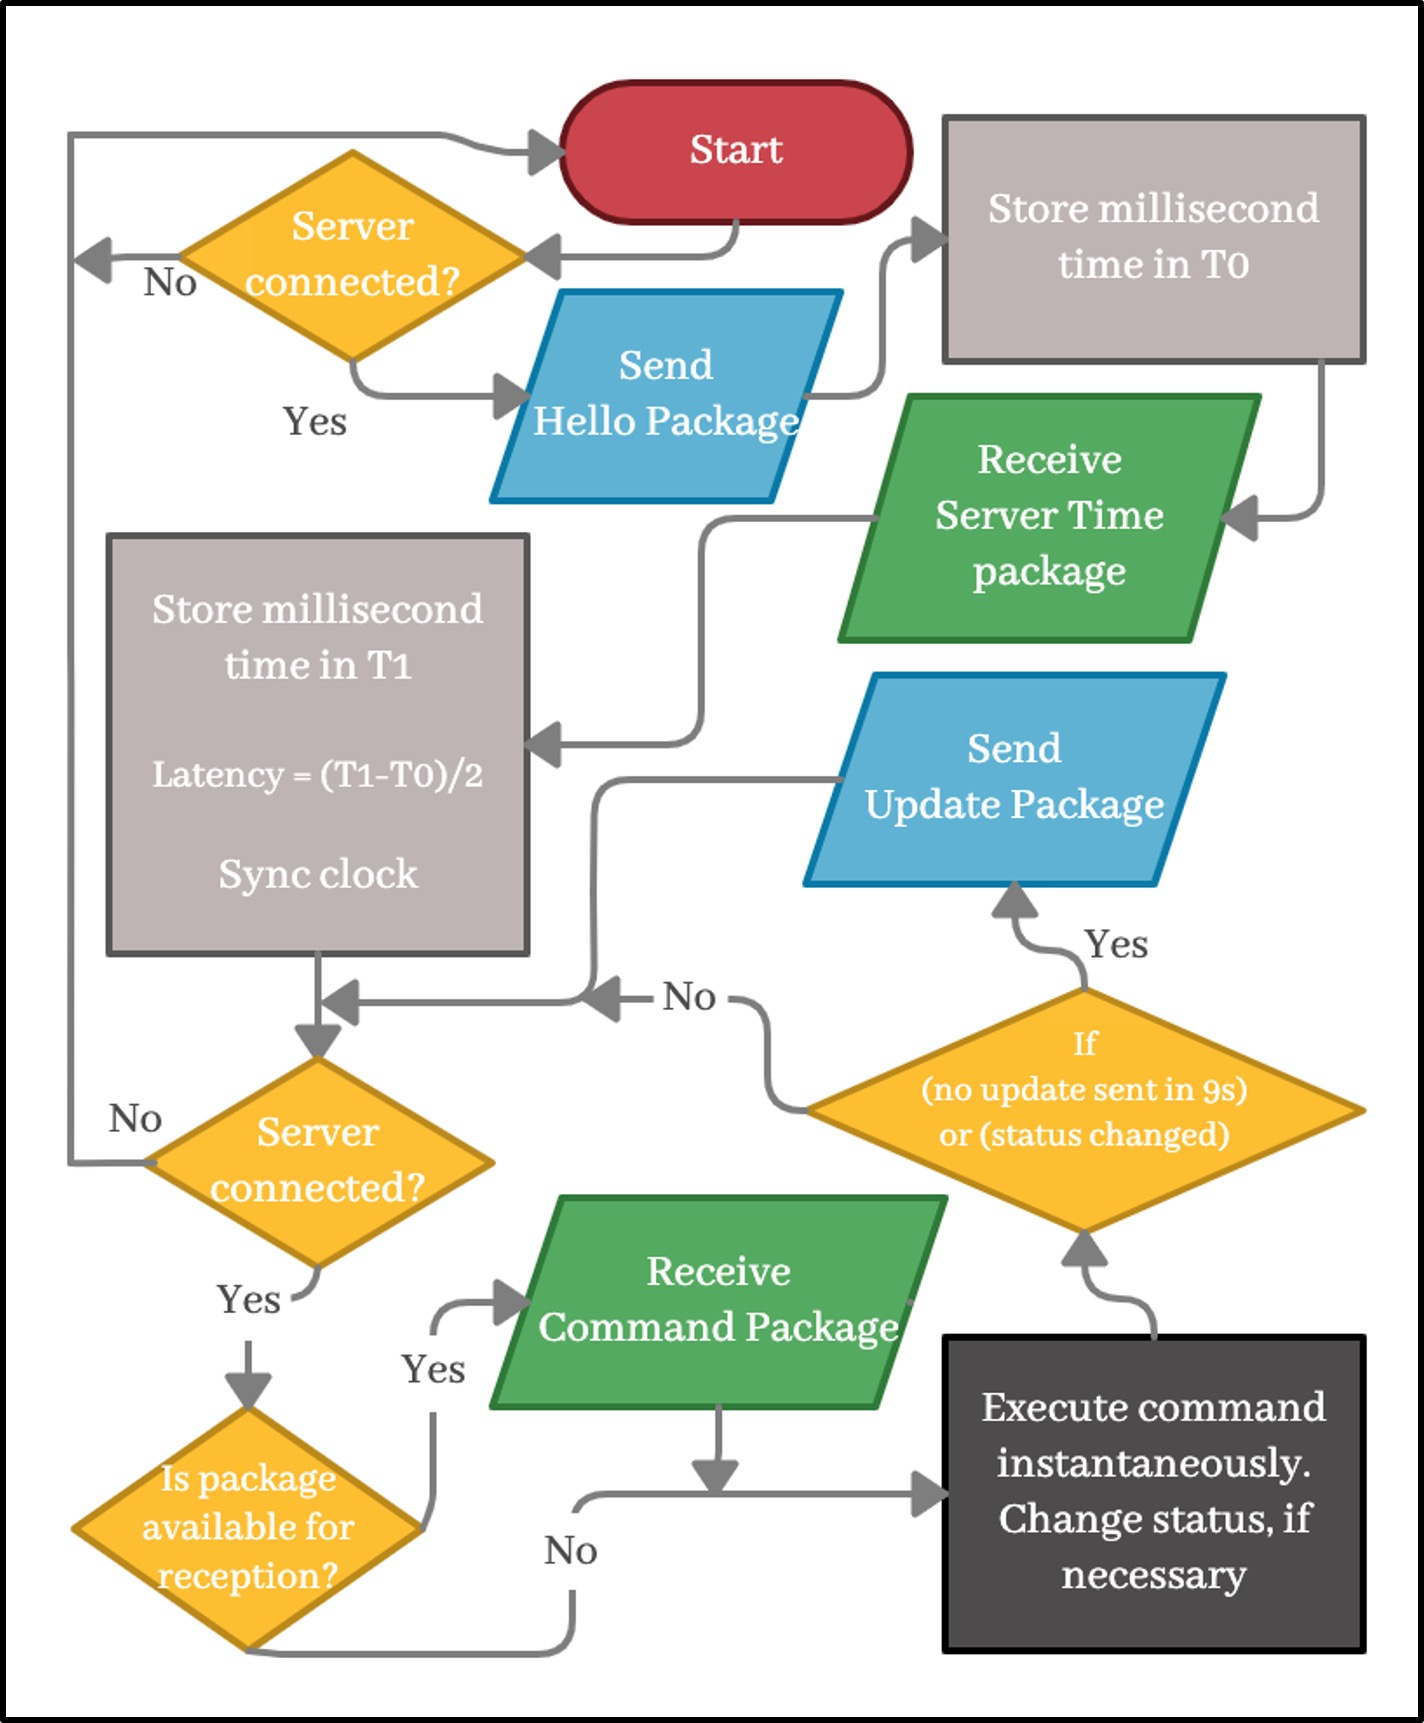
\includegraphics[width=0.485\textwidth]{media/Firmware.jpg}
   \caption{\label{fig_firmware} Simplified Firmware Flow}
\end{figure}

\subsubsection{Executing Commands}
Due to the nature of the constant loop system, commands are "instantaneously" executed as the main loop runs. As a result, motor actions like Sinusoidal Motion and Position-Velocity motion need to be implemented to work in a loop, instead of executing till the motion's completion. This was done using \textit{Bang-Bang Motor Control} and a \textit{Closed-loop Design}.

\begin{enumerate}
    \item \textbf{Bang-Bang Motor Control:} A limitation of the Actuonix L-12I motor is that when it is instructed to move in small increments, it only physically moves when the difference between actual elongation and desired elongation is greater than 5mm. This makes it difficult to implement sinusoidal movement as well as low-velocity movement, as the motor actuates in a repetitive start-stop manner. In order to override this 5mm tolerance and force motor movement, it was decided to instead only alternate motor movement between complete retraction and complete expansion until the desired length is achieved.
    \item \textbf{Closed-loop Design:} For commands like Sinusoidal motion and Position-Velocity control, instead of directly writing the final stroke-length to the motor, intermediate lengths are calculated and written. In each "instantaneous" movement, the desired elongation is calculated by plugging in $t$ (i.e. the time passed since the start of the command) into a function that gives the desired stroke-length, which the motor moves towards using Bang-bang control.
\end{enumerate}

The combination of Bang-Bang control and the Closed-loop design makes the seemingly parallel receiving and execution of commands possible.

\section{Simulation}
In addition to our physical Robot Metabolism prototype, we developed a simulation environment that allows us to explore large numbers of links. The simulation is based on the the Titan library \cite{TitanICRA}. We adapted the library for our application by implementing magnetic interactions between all masses, as well as the necessary controls to activate and deactivate the magnetic interaction. Furthermore, we implemented actuated springs that can expand and contract as our Robot Metabolism links do.

Our simulation was able to simulate over 2000 links with five frames-per-second performance. The magnet interaction calculation is optimized by only considering the relevantly close masses in the calculation via an occupancy grid. As a next step, we are implementing a visualization for the simulation masses as spheres and springs as cylinders, and casts shadows to provide a better scene understanding.

\section{Experiments}

\subsection{Physical Robot Prototype Experiments} To demonstrate the capability of the Robot Metabolism we intend to perform two experiments.
\subsubsection{Herbivore} First, we will study the capacity of a Robot Metabolism assembly to act as a Herbivore that is harvesting found resources, and uses them to improve itself. In this scenario, a crawling tetrahedron will find an abandoned robot link, and integrate it in such a way that the tetrahedron forms a pusher configuration and can change its gate.
\subsubsection{Carnivore} Second, we will explore the capability of a Robot Metabolism assembly to act as a carnivore that conquers other robot-metabolism assemblies and uses their parts to improve itself. For example a tetrahedron that encounters a triangle and uses the newly gained parts to improve itself.

\subsection{Simulation Experiments}
There are two types of simulations that we would like to to explore with respect to this robot concept. First, a high-fidelity simulation with a low simulation-reality-gap that allows us to test a hypothesis in simulation before trying it on the robot platform. Second, we would like a high-performance, parallelized simulation that allows us to run experiments with thousands of virtual robot links for the study of the origin of life.
\subsubsection{Simulation: Hypothesis testing}
We require a simulation that ties into our Robot Metabolism Eco-system in such a way that virtual links can connect to the robot server as if they were physical links, and be commanded via the same package commands as their physical counter parts. This way we can test our algorithms in simulation and then run the same code without modifications to command the physical robots.
\subsubsection{Simulation: Origin Of Life}
We would like to study the origin of life by allowing random populations of robot links to interact with each other and copy their controllers to other links. Our exploration is inspired by Studer et. al.'s findings in the "Spontaneous Emergence of Self-Replicating Structures in Molecube Automata" \cite{Studer2006}.  We would like to replicate their findings in 3D using our Robot Metabolism simulation.

\section{Conclusion}
This semester, we have built three links of our simplified design. We further refined our wiring and on-board power management of the link prototype: each link has accessible LiPo batteries for easy recharging, as well as a battery hole cover. We have completed the implementation of our Robot Link firmware, and implemented a server that can connect to and command the Robot Links. Further, we successfully ran a walking tetrahedron experiment script that by interacting with the server, made three Robot Links crawl across a shaggy carpet in a triangle formation. This semester we laid the ground work that makes Robot Metabolism a working experiment platform.
\section{Future Work}
As a next step we want to assemble eight Robot Metabolism links, and show that a basic link structure can metabolize other links or even other substructures to improve itself. To achieve this goal we will have to develop a simulation environment to evolve possible movement patterns that lead to a successful pickup of new links. Simulatenously, we can attempt to handcode a solution for the Herbivor experiment. Additionally, in an effort to research the origin of life, we are going to run an experiment where a number of robot links randomly crawl, or execute motions on a plane. We then observe if they form a simple sub-structure by chance. If substructures are randomly formed, we will quantify how rare/frequent the occurrence of a basic sub-structure is. Finally, we are aiming to build 15 robot metabolism to allow for more complex experiments.


\addtolength{\textheight}{-12cm}   % This command serves to balance the column lengths
                                  % on the last page of the document manually. It shortens
                                  % the textheight of the last page by a suitable amount.
                                  % This command does not take effect until the next page
                                  % so it should come on the page before the last. Make
                                  % sure that you do not shorten the textheight too much.

%%%%%%%%%%%%%%%%%%%%%%%%%%%%%%%%%%%%%%%%%%%%%%%%%%%%%%%%%%%%%%%%%%%%%%%%%%%%%%%%



%%%%%%%%%%%%%%%%%%%%%%%%%%%%%%%%%%%%%%%%%%%%%%%%%%%%%%%%%%%%%%%%%%%%%%%%%%%%%%%%



%%%%%%%%%%%%%%%%%%%%%%%%%%%%%%%%%%%%%%%%%%%%%%%%%%%%%%%%%%%%%%%%%%%%%%%%%%%%%%%%

\section{ACKNOWLEDGMENT}

Thanks to DARPA Trades for funding this research. 
U.S. Defense Advanced Research Project Agency (DARPA) TRADES grant number HR0011-17-2-0014.


\section{Who Did What?}
\begin{table}[htbp]
\caption{Dataset specification table}
\begin{center}
\begin{tabular}{llll}
\textbf{Task}                       & \rotatebox[origin=c]{75}{\textbf{Philippe Wyder}} & \rotatebox[origin=c]{75}{\textbf{Riyaan Bakhda}} & \rotatebox[origin=c]{75}{\textbf{Nihar Garg}} \\
Conceptualization                   & x              &               &            \\
Prototype Design                    & x              &               &            \\
Experiment Design                   & x              &               &            \\
Experiment Walking Triangle         & x              & x             &            \\
Building Robot Links                &                &               & x          \\
Ordering / Administration           & x              &               &            \\
Hiring \& Training                  & x              &               &            \\
Documenting Prototype Build Process &                &               & x          \\
Implementing Robot Link Firmware    & x              & x             &            \\
Designing RMLProtocol              & x              & x             &            \\
Implementing RMLProtocol            &                & x             &            \\
Implementing Link Server            &                & x             &            \\
Implementing Build Scripts          &                & x             &            \\
Documenting Software                & x              & x             &            \\
Robot Control Code                  &                & x             &           
\end{tabular}
\end{center}
\end{table}
%%%%%%%%%%%%%%%%%%%%%%%%%%%%%%%%%%%%%%%%%%%%%%%%%%%%%%%%%%%%%%%%%%%%%%%%%%%%%%%%



\bibliographystyle{ieeetr}
\bibliography{references}

\newpage
\appendix
\section{Appendices}

\subsection{Build Process}

%\href{run:media/buildprocess_v1.pdf}{Link to PDF}

\href{https://docs.google.com/document/d/1_NFA3L7FgsLT_E70pb2BcXp33b8JFPGKjbd9sz8ftQI/edit?usp=sharing}{Link to Google Doc: https://bit.ly/32ttSeU}

\subsection{RMLProtocol Definition}

\href{https://docs.google.com/document/d/1cSnrM0hEOot5myDe9eK7aO5bT6LY-UzJp4RNLIoQbEQ/edit?usp=sharing}{Link to Google Doc: https://bit.ly/2QXqoic}


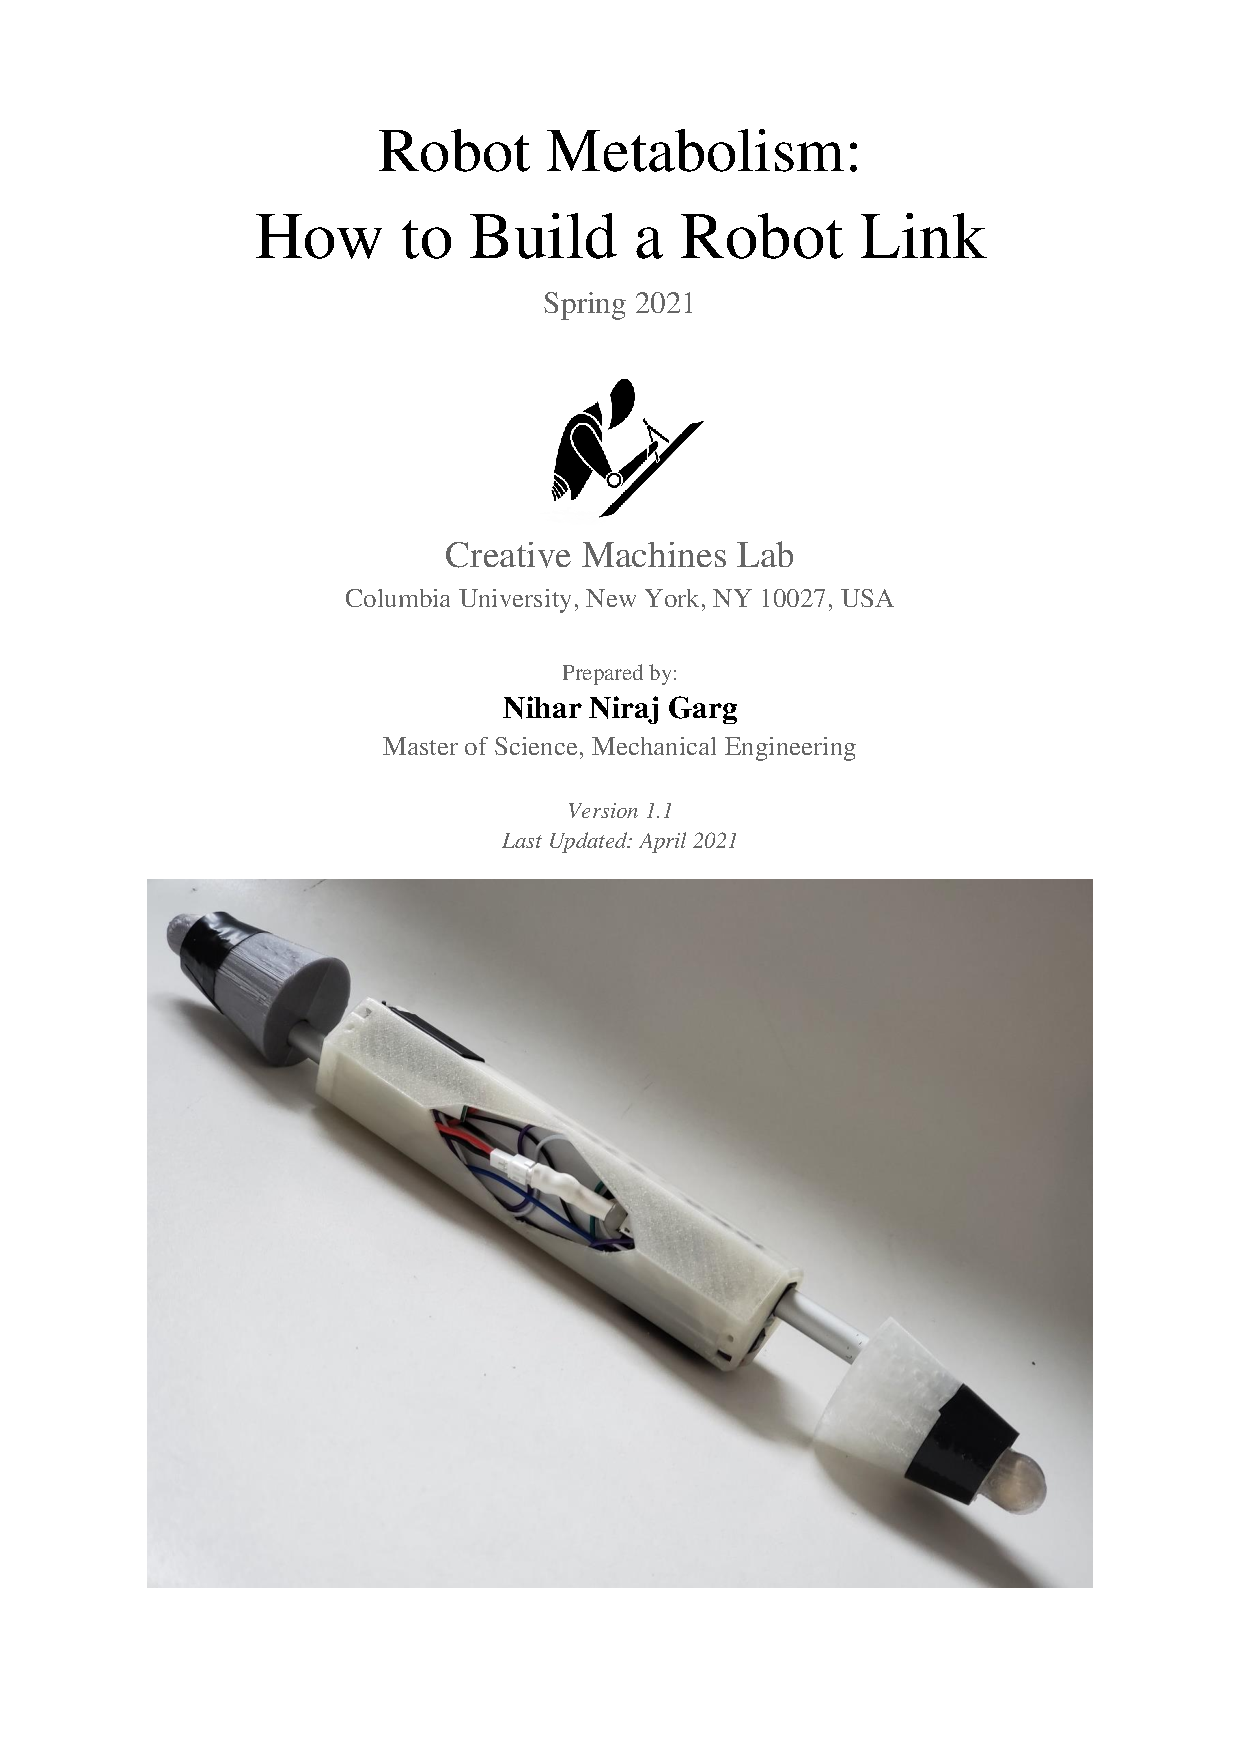
\includepdf[pages=-,pagecommand={},width=\textwidth]{media/BuildProcess_v1.pdf}

\newpage
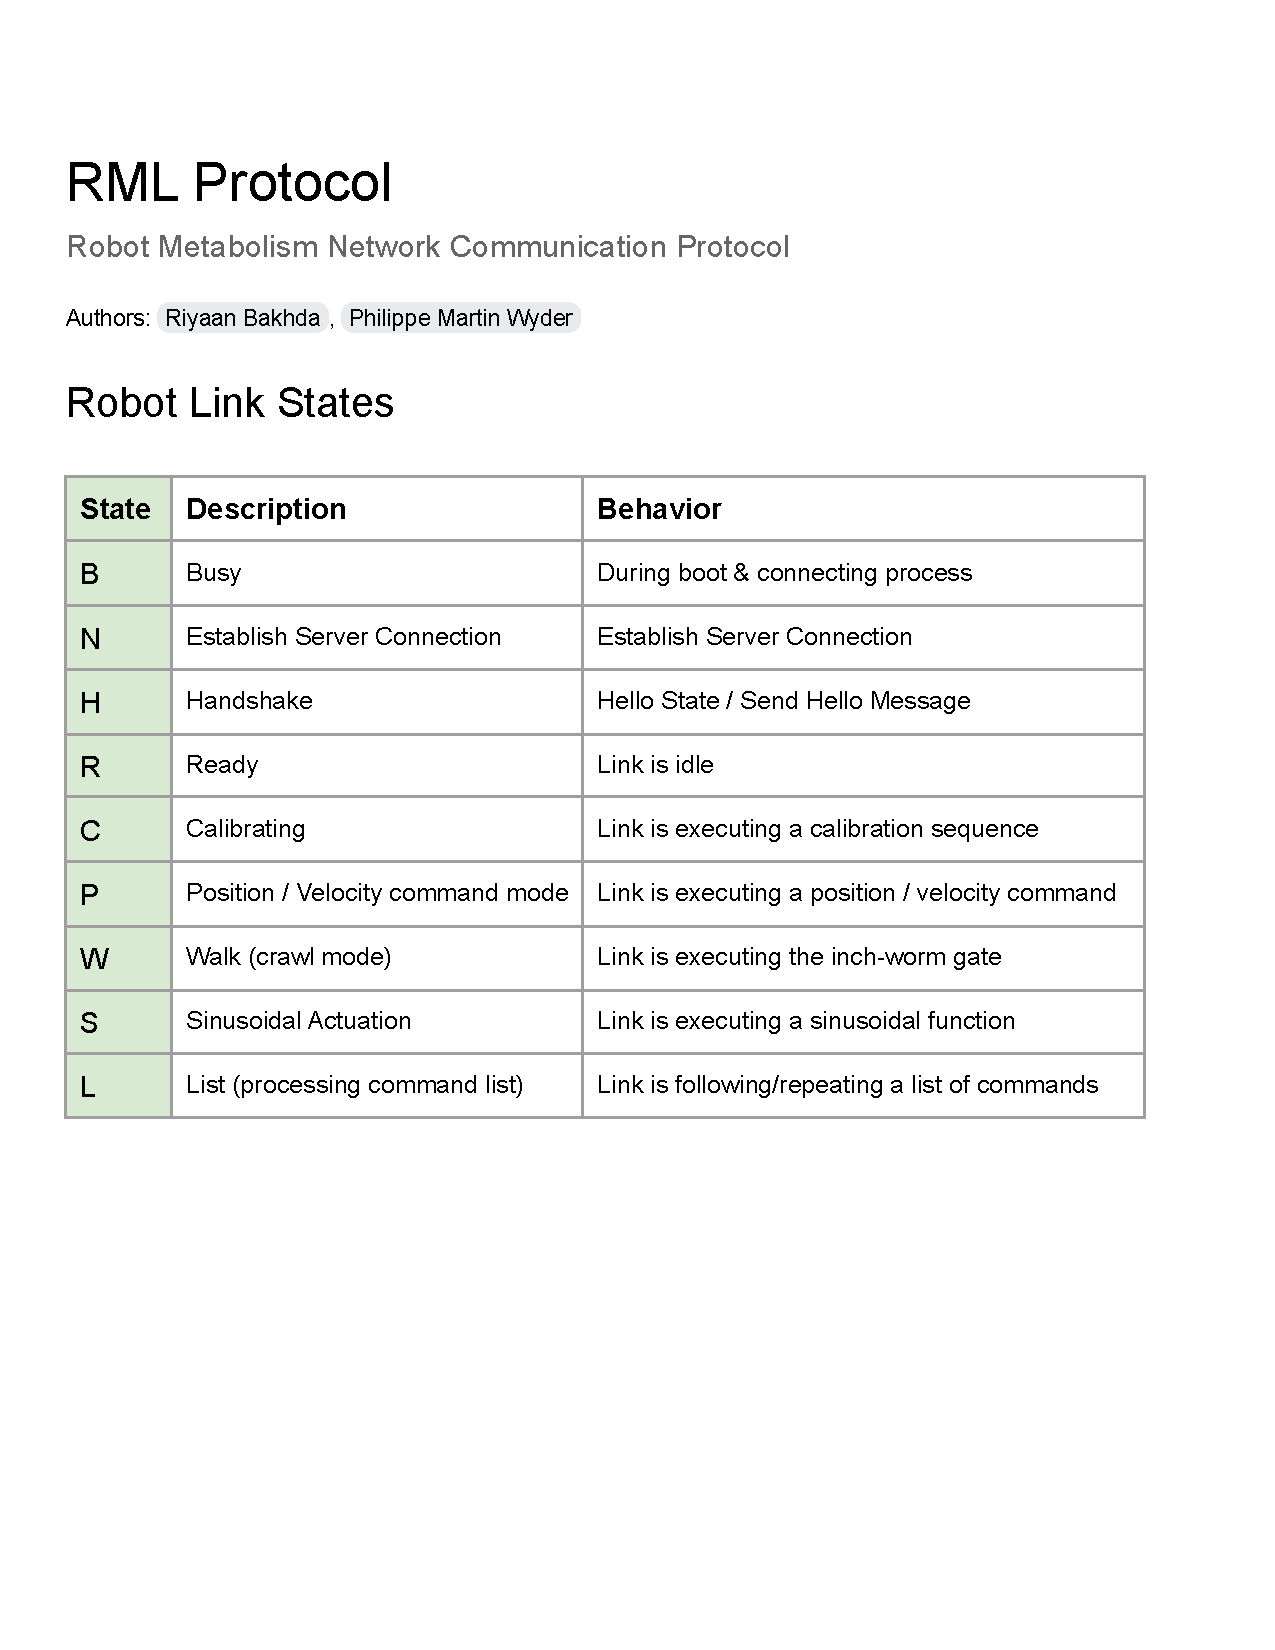
\includepdf[pages=-,pagecommand={},width=\textwidth]{media/RML_Protocol.pdf}

\end{document}
